% Created 2021-04-12 Mon 13:11
% Intended LaTeX compiler: pdflatex

\documentclass[oneside]{book}
\usepackage[T1, T2A]{fontenc}
\usepackage[lutf8]{luainputenc}
\usepackage[english, russian]{babel}
\usepackage{minted}
\usepackage{graphicx}
\usepackage{longtable}
\usepackage{hyperref}
\usepackage{xcolor}
\usepackage{natbib}
\usepackage{amssymb}
\usepackage{stmaryrd}
\usepackage{amsmath}
\usepackage{caption}
\usepackage{mathtools}
\usepackage{amsthm}
\usepackage{tikz}
\usepackage{grffile}
\usepackage{extarrows}
\usepackage{wrapfig}
\usepackage{algorithm}
\usepackage{algorithmic}
\usepackage{lipsum}
\usepackage{rotating}
\usepackage{placeins}
\usepackage[normalem]{ulem}
\usepackage{amsmath}
\usepackage{textcomp}
\usepackage{capt-of}

\addto\captionsrussian{\renewcommand{\chaptername}{Лекция}}
 \usepackage{hyperref}
 \hypersetup{
     colorlinks=true,
     linkcolor=blue,
     filecolor=orange,
     citecolor=black,      
     urlcolor=cyan,
     }

\usetikzlibrary{decorations.markings}
\usetikzlibrary{cd}
\usetikzlibrary{patterns}
\usetikzlibrary{automata, arrows}

\newcommand\addtag{\refstepcounter{equation}\tag{\theequation}}
\newcommand{\eqrefoffset}[1]{\addtocounter{equation}{-#1}(\arabic{equation}\addtocounter{equation}{#1})}
\newcommand{\llb}{\llbracket}
\newcommand{\rrb}{\rrbracket}


\newcommand{\R}{\mathbb{R}}
\renewcommand{\C}{\mathbb{C}}
\newcommand{\N}{\mathbb{N}}
\newcommand{\A}{\mathfrak{A}}
\newcommand{\B}{\mathfrak{B}}
\newcommand{\rank}{\mathop{\rm rank}\nolimits}
\newcommand{\const}{\var{const}}
\newcommand{\grad}{\mathop{\rm grad}\nolimits}

\newcommand{\todo}{{\color{red}\fbox{\text{Доделать}}}}
\newcommand{\fixme}{{\color{red}\fbox{\text{Исправить}}}}

\newcounter{propertycnt}
\setcounter{propertycnt}{1}
\newcommand{\beginproperty}{\setcounter{propertycnt}{1}}

\theoremstyle{plain}
\newtheorem{propertyinner}{Свойство}
\newenvironment{property}{
  \renewcommand\thepropertyinner{\arabic{propertycnt}}
  \propertyinner
}{\endpropertyinner\stepcounter{propertycnt}}
\newtheorem{axiom}{Аксиома}
\newtheorem{lemma}{Лемма}
\newtheorem{manuallemmainner}{Лемма}
\newenvironment{manuallemma}[1]{%
  \renewcommand\themanuallemmainner{#1}%
  \manuallemmainner
}{\endmanuallemmainner}

\theoremstyle{remark}
\newtheorem*{remark}{Примечание}
\newtheorem*{solution}{Решение}
\newtheorem{corollary}{Следствие}[theorem]
\newtheorem*{examp}{Пример}
\newtheorem*{observation}{Наблюдение}

\theoremstyle{definition}
\newtheorem{task}{Задача}
\newtheorem{theorem}{Теорема}[section]
\newtheorem*{definition}{Определение}
\newtheorem*{symb}{Обозначение}
\newtheorem{manualtheoreminner}{Теорема}
\newenvironment{manualtheorem}[1]{%
  \renewcommand\themanualtheoreminner{#1}%
  \manualtheoreminner
}{\endmanualtheoreminner}
\captionsetup{justification=centering,margin=2cm}
\newenvironment{colored}[1]{\color{#1}}{}

\tikzset{->-/.style={decoration={
  markings,
  mark=at position .5 with {\arrow{>}}},postaction={decorate}}}
\makeatletter
\newcommand*{\relrelbarsep}{.386ex}
\newcommand*{\relrelbar}{%
  \mathrel{%
    \mathpalette\@relrelbar\relrelbarsep
  }%
}
\newcommand*{\@relrelbar}[2]{%
  \raise#2\hbox to 0pt{$\m@th#1\relbar$\hss}%
  \lower#2\hbox{$\m@th#1\relbar$}%
}
\providecommand*{\rightrightarrowsfill@}{%
  \arrowfill@\relrelbar\relrelbar\rightrightarrows
}
\providecommand*{\leftleftarrowsfill@}{%
  \arrowfill@\leftleftarrows\relrelbar\relrelbar
}
\providecommand*{\xrightrightarrows}[2][]{%
  \ext@arrow 0359\rightrightarrowsfill@{#1}{#2}%
}
\providecommand*{\xleftleftarrows}[2][]{%
  \ext@arrow 3095\leftleftarrowsfill@{#1}{#2}%
}
\makeatother

\newenvironment{rualgo}[1][]
  {\begin{algorithm}[#1]
     \selectlanguage{russian}%
     \floatname{algorithm}{Алгоритм}%
     \renewcommand{\algorithmicif}{{\color{red}\textbf{если}}}%
     \renewcommand{\algorithmicthen}{{\color{red}\textbf{тогда}}}%
     \renewcommand{\algorithmicelse}{{\color{red}\textbf{иначе}}}%
     \renewcommand{\algorithmicend}{{\color{red}\textbf{конец}}}%
     \renewcommand{\algorithmicfor}{{\color{red}\textbf{для}}}%
     \renewcommand{\algorithmicto}{{\color{red}\textbf{до}}}%
     \renewcommand{\algorithmicdo}{{\color{red}\textbf{делать}}}%
     \renewcommand{\algorithmicwhile}{{\color{red}\textbf{пока}}}%
     \renewcommand{\algorithmicrepeat}{{\color{red}\textbf{повторять}}}%
     \renewcommand{\algorithmicuntil}{{\color{red}\textbf{до тех пор пока}}}%
     \renewcommand{\algorithmicloop}{{\color{red}\textbf{повторять}}}%
     \renewcommand{\algorithmicnot}{{\color{blue}\textbf{не}}}%
     \renewcommand{\algorithmicand}{{\color{blue}\textbf{и}}}%
     \renewcommand{\algorithmicor}{{\color{blue}\textbf{или}}}%
     \renewcommand{\algorithmicrequire}{{\color{blue}\textbf{Предусловие}}}%
     \renewcommand{\algorithmicrensure}{{\color{blue}\textbf{Постусловие}}}%
     \renewcommand{\algorithmicrtrue}{{\color{blue}\textbf{истинна}}}%
     \renewcommand{\algorithmicrfalse}{{\color{blue}\textbf{ложь}}}%
     % Set other language requirements
  }
  {\end{algorithm}}
\author{Ilya Yaroshevskiy}
\date{\today}
\title{Лекции по Математическому анализу 4 семестр}
\hypersetup{
 pdfauthor={Ilya Yaroshevskiy},
 pdftitle={Лекции по Математическому анализу 4 семестр},
 pdfkeywords={},
 pdfsubject={},
 pdfcreator={Emacs 28.0.50 (Org mode 9.4.4)}, 
 pdflang={English}}
\begin{document}

\maketitle
\tableofcontents



\chapter{}
\label{sec:org7ee6692}
\renewcommand{\P}{\mathcal{P}}
\newcommand{\A}{\mathfrak{A}}
\newcommand{\B}{\mathfrak{B}}
\newcommand{\M}{\mathfrak{M}}

\section{Теория меры}
\label{sec:orge972367}
\begin{lemma}[о структуре компактного оператора]
\(V : \R^m \to \R^m\) --- невырожденный линейный оператор, т.е. \(\det V \neq 0\) \\
\uline{Тогда}:
\begin{itemize}
\item \(\exists\) ортонормированные базисы \(g_1, \dots, g_m;\ h_1, \dots, h_m\)
\item \(\exists S_1, \dots, S_m > 0\)
\end{itemize}
\[ \forall x \in \R^m\quad V(x) = \sum_{i = 1}^m S_i \langle x, g_i \rangle h_i$ \]
\color{gray} \(x = \sum \langle x, g_i \rangle g_i\) --- разложение по базису \color{black} \\
\textbf{При этом} \(\vert\det V\vert = S_1 S_2 \dots S_m\)
\label{org098c67b}
\end{lemma}
\begin{proof}
\(W := V^*V\) \color{gray} * --- транспонирование в \(\R^m\) \color{black} \\
\color{gray} \(W\) --- самосопряженный оператор(матрица симметрична относительно диагонали) \color{black} \\
Собственные числа \(c_1, \dots, c_m\) --- вещественные \\
Собственные векторы \(g_1, \dots, g_m\) \\
Заметим что \(c_i\langle g_i, g_i \rangle = \langle Wg_i, g_i \rangle = \langle Vg_i, Vg_i \rangle > 0 \Rightarrow c_i > 0\) \\
\begin{itemize}
\item \(S_i := \sqrt{c_i}\) \\
\item \(h_i := \frac{1}{S_i} Vg_i\) \\
\end{itemize}
\[ \langle h_i, h_j \rangle = \frac{1}{S_iS_j}\langle Vg_i, Vg_j\rangle = \frac{1}{S_iS_j}\langle Wg_i, g_j\rangle = \frac{c_i}{S_iS_j}\langle g_i, g_j \rangle = \delta_i \]
\[ V(x) = V(\sum_{i=1}^n\langle x, g_i \rangle g_i) = \sum_{i = 1}^m \langle x, g_i \rangle V(g_i) = \sum s_i \langle x, g_i \rangle h_i \]
\[ (\det V)^2 = \det(V^*V) = \det W = c_1\dots c_m \addtag\label{diag_1} \]
\(\ref{diag_1}\) --- т.к. диагональная матрица
\label{orgab4c889}
\end{proof}
\begin{theorem}[преобразование меры лебега при линейном отображении]
\-
\begin{itemize}
\item \(V: \R^m \to \R^m\) --- линейное отображение
\end{itemize}
\uline{Тогда}:
\begin{itemize}
\item \(\forall E \in \M^m\quad V(E) \in \M^m\)
\item \(\lambda(V(E)) = \vert \det V \vert \cdot \lambda E\)
\end{itemize}
\label{org95549ba}
\end{theorem}
\begin{proof}
\- 
\begin{description}
\item[{(\(\det V = 0\))}] \(\text{Im}(V)\) --- подпространство в \(\R^m\) \(\Rightarrow\) мера \(=0\)
\item[{(\(\det V \neq 0\))}] \(\mu E := \lambda(V(E))\) --- мера \\
\(\mu\) --- инвариантна относительно сдвигов
\[ \mu(E + a) = \lambda(V(E + a)) = \lambda(V(E) + Va) = \lambda(V(E)) = \mu E \]
\(\Rightarrow\) \(\exists k: \mu = k\cdot \lambda\)(Лемма из предыдущего семестра) \\
\(Q\) --- единичный куб на векторах \(g_i\) и \(V(g_i) = S_ih_i\), \(V(Q) = \{\sum\alpha_iS_ih_i \vert \alpha_i \in [0,1]\}\) --- паралеллепипед со сторонами \(S_i, \dots, S_m\)
\end{description}
\label{org8601846}
\end{proof}
\section{Интеграл}
\label{sec:orgad9d5a9}
\subsection{Измеримые функции}
\label{sec:orgee40c1d}
\begin{definition}
\-
\begin{enumerate}
\item \(E\) --- множество, \(E = \underset{\text{кон.}}{\bigsqcup}e_i\) --- \textbf{разбиение множества}
\item \(f: X \to \R\) --- \textbf{ступенчатая}, если \\
\(\exists\) разбиение \(X = \underset{\text{кон.}}{\bigsqcup}e_i:\ \forall i\ f\big\vert_{e_i} = \const = c_i\) \\
При этом такое разбиение --- \textbf{допустимое разбиение}
\end{enumerate}
\label{org6325d0f}
\end{definition}
\begin{examp}
\-
\begin{enumerate}
\item Характеристическая функция множества \(E \subset \mathcal{X}_E(x) = \left[\begin{array}{ll} 1 & x \in E \\ 0 & x \in X \setminus E \end{array}\)
\item \(f = \subset{\text{кон.}}{\sum}c_i\mathcal{X}_{e_i}\), где \(\mathcal{X} = \bigsqcup e_i\)
\end{enumerate}
\label{org1b7295b}
\end{examp}
\begin{remark}
\-
\begin{enumerate}
\item \(\forall f, g\) --- ступенчатые \\
\uline{Тогда} \(\exists\) разбиения, допутимые и для \(f\), и для \(g\) \\
\[ f = \sum_\text{кон.} c_i \mathcal{X}_{e_i}\quad h = \sum_\text{кон.} b_k \mathcal{X}_{A_k} \]
\[ f = \sum_{i, k} c_i \mathcal{X}_{e_i\cap A_k} \quad g = \sum b_k\cdot\mathcal{X}_{e_i \cap A_k} \]
\item \(f, g\) --- ступенчатые, \(\alpha \in \R\) \\
\uline{Тогда} \(f + g,\ \alpha f,\ fg,\ max(f, g),\ min(f, g),\ |f|\) --- ступенчатые
\end{enumerate}
\label{org73b9e8e}
\end{remark}
\begin{definition}
\(f: E\subset X \to \overline{\R},\ a \in \R\) \\
\(E(f < a) = \{x\in E: f(x) < a\}\) --- \textbf{лебегово множество функции \(f\)} \\
\(E(f \le a),\ E(f > a), E(f \ge a)\) --- также лебеговы множества \\
Если \(f\) задана на \(X\): \(X(f < a),\ X(f \le a), \dots\) --- лебеговы множества
\label{orgbbf5c6d}
\end{definition}
\begin{remark}
\(E(f \ge a) = E(f < a)^C;\ E(f < a) = E(f \ge a)^C\) \\
\[ E(f \le a) = \bigcap_{b > a} E(f < b) = \bigcap_{n \in \N}E(f < a + \frac{1}{n})\]
\label{org88d9991}
\end{remark}
\begin{definition}
\-
\begin{itemize}
\item \((X, \A, \mu)\) --- пространство с мерой
\item \(f: X \to \overline{\R}\)
\item \(E \in \A\)
\end{itemize}
\(f\) --- \textbf{измерима на множестве \(E\)}: \\
\(a \in \R\quad E(f < a)\) --- измеримо(т.е. \(\in \A\))
\label{org073efac}
\end{definition}
\begin{symb}
\-
\begin{itemize}
\item \(f\) --- измеримо на \(X\) --- говорят просто "измеримо"
\item \(X = \R^m\), мера Лебега --- измеримо по Лебегу
\end{itemize}
\label{org9d58d0d}
\end{symb}
\begin{remark}
Эквивалентны:
\begin{enumerate}
\item \(\forall a\quad E(f < a)\) --- измеримо
\item \(\forall a\quad E(f \le a)\) --- измеримо
\item \(\forall a\quad E(f > a)\) --- измеримо
\item \(\forall a\quad E(f \ge a)\) --- измеримо
\end{enumerate}
\label{org7fa37d8}
\end{remark}
\begin{examp}
\begin{enumerate}
\item \(E \subset X\), \(E\) --- измеримо, \(\mathcal{X}_E\) --- измеримо \\
\(E(\mathcal{X}_E < a) = \left[\begin{array}{ll} \emptyset & ,a < 0 \\ X \setminus E & ,0 <= a <= 1 \\ X & ,a > 1 \end{array}\)
\item \(f: \R^m \to \R\) --- непрерывна. Тогда \(f\) --- измеримо по Лебегу
\end{enumerate}
\label{orgba9e6ee}
\end{examp}
\begin{remark}
\emph{Свойства}:
\begin{enumerate}
\item \(f\) --- измерима на \(E\)
\begin{description}
\item[{\(\Rightarrow\)}] \(\forall a \in \R\) \(E(f = a)\) --- измеримо \\
\item[{\(\not \Leftarrow\)}] \(f: \R \to \R\quad f(x) = \mathcal{X} + \mathcal{X}_\text{неизм.}\)
\end{description}
\item \(f\) --- измерима \(\Rightarrow\) \(\forall \alpha \in R\quad \alpha f\) --- измерима
\item \(f\) --- измерима \(E_1, E_2, \dots \Rightarrow f\) --- измерима на \(E = \bigcup E_k\)
\item \(f\) --- измерима на \(E\); \(\underset{\text{изм.}}{E'} \subset E \Rightarrow f\) --- измерима на \(E'\) \\
\(E'(f < a) = E(f < a) \cap E'\)
\item \(f \neq 0\) --- измерима на \(E\) \(\Rightarrow\) \(\frac{1}{f}\) --- измерима на \(E\)
\item \(f \ge 0\), измерима на \(E\), \(\alpha \in \R\). \uline{Тогда} \(f^\alpha\) --- измерима на \(E\)
\end{enumerate}
\label{org23889b0}
\end{remark}
\begin{theorem}
\(f_n\) --- измерима на \(X\). \\
\uline{Тогда}:
\begin{enumerate}
\item \[ \sup_{n \in \N} f_n;\quad \inf_{n \in \N} f_n \addtag\label{sup_inf_1} \]
\(\ref{sup_inf_1}\) --- измеримы
\item \(\overline{\lim} f_n;\quad\underline{\lim} f_n\) --- измеримы
\item Если \[ \forall x\ \exists \lim_{n \to +\infty}f_n(x) = h(x) \], то \(h(x)\) --- измеримо
\end{enumerate}
\label{org225823d}
\end{theorem}
\begin{proof}
\-
\begin{enumerate}
\item \(g = \sup f_n\quad X(g > a) = \bigcup X(f_n > a)\)
\item \[ (\overline{\lim} f_n)(x) = \inf\{s_n: s_n = \sup(f_n(x), f_{n + 1}(x), \dots)\} \]
\item очев.
\end{enumerate}
\label{org1c3997e}
\end{proof}

\subsection{Меры Лебега-Стильеса}
\label{sec:org1e237c8}
\begin{definition}
\(\R, \P^1, g:\R \to \R\) --- возрастает, непрерывна \\
\(\mu[a, b) := g(b) - g(a)\) --- \(\sigma\)-конечный объем \\
\[ g(a + 0) = \lim_{x \to a + 0}g(x), g(a - 0) = \lim_{x \to a - 0}g(x) \]
\[ \mu[a, b) := g(b-0) - g(a - 0) \]
--- тоже \(\sigma\)-конечная мера \\
Применим теорему о продолжении, получим меру \(\mu g\) на некой \(\sigma\)-алгебре --- \textbf{мера Лебега-Стилтьеса} 
\label{org8440af8}
\end{definition}
\begin{definition}
\(g(x) = \lceil x \rceil\) \\
Пусть \(\mu g\) определена на Борелевской \(\sigma\)-алгебре --- \textbf{мера Бореля-Стилтьеса}
\label{org25ac6a7}
\end{definition}
\chapter{}
\label{sec:org5cbcfe0}
\newcommand{\X}{\mathcal{X}}
\newcommand{\A}{\mathfrak{A}}

\section{Теореия меры}
\label{sec:org2ffcba2}
\subsection{Измеримые функции}
\label{sec:orga7de7b4}
\begin{itemize}
\item \((X, \A, \mu)\)
\item \(f: X \to \overline{R}\) имзмерима
\item \(\forall a \in R\quad X(f < a) \in \A\)
\item \(\X_E\quad \sum \alpha_k \X_{E_k}\)
\end{itemize}
\begin{theorem}[характеризация измеримости функции с помощью ступенчатых]
\-
\begin{itemize}
\item \(f: X \to \overline{R}\)
\item \(f \ge 0\)
\item \(f\) --- измерима
\end{itemize}
\uline{Тогда} \(\exists f_n\) --- ступенчатая
\begin{enumerate}
\item \(0 \le f_1 \le f_2 \le \dots\)
\item \(\forall x f(x) = \lim_{n \to + \infty}f_n(x)\)
\end{enumerate}
\label{orga36c50e}
\end{theorem}
\begin{proof}
\begin{center}
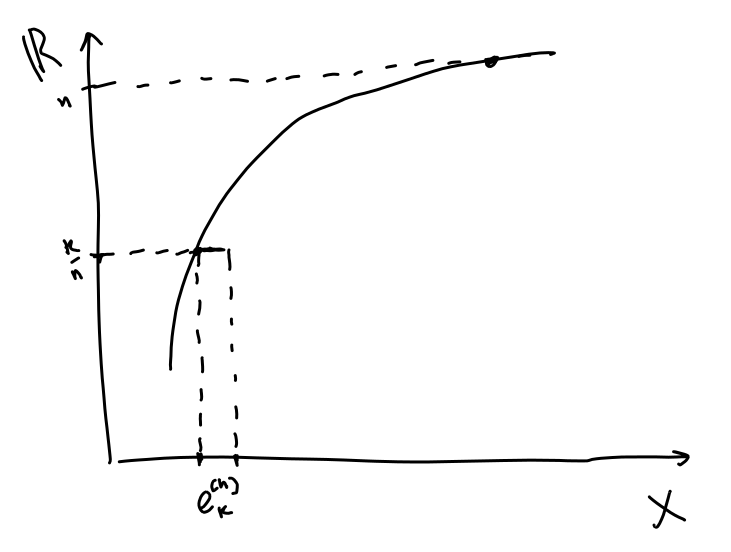
\includegraphics[scale=0.5]{2_1.png}
\end{center}
\[ e^{(n)}_k = X(\frac{k - 1}{n} \le f \le \frac{k}{n}) \quad k = 1,\dots,n^2 \]
\[ e^{(n)}_{n^2 + 1} = X(n \le f) \]
\[ g_n := \sum^{n + 1}_{k = 1} \frac{k - 1}{n} \X_{e^{(n)}_k} \]
\[ g_n \ge 0 \quad \lim_{n \to + \infty}g_n(x) = f(x) \]
\label{org322b387}
\end{proof}
\begin{corollary}
\(f\) --- имзерима \\
\uline{Тогда} \(\exists f_n\) --- ступенчатая, \(f_n \xrightarrow{n \to + \infty}{} f\) всюду и \(|f_n| \le |f|\)
\label{orga9b778e}
\end{corollary}
\begin{corollary}
\(f, g\) --- измеримы \\
\uline{Тогда} \(fg\) --- измемрима (\(0\cdot\infty=0\))
\label{org10ef661}
\end{corollary}
\begin{proof}
\(f_n \to f\quad g_n \to g\), (\(f_n, g_n\)) --- ступеначтые \\
\(f_ng_n\) --- ступенчатая \(f_ng_n \to fg\)
\label{org7e2befe}
\end{proof}
\begin{corollary}
\(f, g\) --- измеримы \\
\uline{Тогда} \(f + g\) --- измерима
\label{orgae41baa}
\end{corollary}
\begin{proof}
\(f_n \to f\quad g_n \to g\), (\(f_n, g_n\)) --- ступеначтые \\
\(f_n + g_n\) --- ступенчатая \(f_n + g_n \to f + g\) \\
\color{gray}Считаем что \(\forall x\), не может быть \(f(x) = \pm \infty,\ g(x) = \mp \infty\)
\label{orgc72f01b}
\end{proof}

\begin{itemize}
\item \(A \subset X\)
\item \(A\) --- полная мера
\item \(\mu(X \setminus A) = 0\)
\end{itemize}
\begin{theorem}[об измеримости непрерывной на множестве полной меры]
\-
\begin{itemize}
\item \(f: E\to\R\)
\item \(E \subset \R^m\)
\item \(e \subset R\)
\item \(\lambda_me = 0\)
\item \(f\) --- непрерывна на \(E' = E \setminus e\)
\end{itemize}
\uline{Тогда} \(f\) --- измерима
\label{org240ca79}
\end{theorem}
\begin{proof}
\(f\) --- измерима на \(E'\)  \\
\(E'(f < a)\) --- открыто в \(E'\) \\
\[ \left.\begin{array}{c} e(f < a) \subset e & \lambda_n \text{ --- полная}\end{array}\right\} \Rightarrow e(f < a)\text{ --- измерима в} E \]
\[ E(f < a) = E'(f < a) \cup e(f < a) \]
\label{orgebcce93}
\end{proof}
\begin{examp}
\-
\begin{itemize}
\item \(E = \R\)
\item \(f = \X_{\text{Irr}}\)
\end{itemize}
\end{examp}
\begin{corollary}
\-
\begin{itemize}
\item \((X, \A, \mu)\)
\item \(f: E\to\R\)
\item \(e \subset E \subset X\)
\item \(E' = E \setminus e\)
\item \(f\) --- измерима на \(E'\)
\end{itemize}
\uline{Тогда} модно так переопределить \(f\) на множестве \(e\), что полученая функция \(\tilde{f}\) будет измерима на \(E\)
\end{corollary}
\begin{proof}
Пусть:
\[ \tilde{f} = \left\{\begin{array}{ll}f(x) & , x \in E \\ \const & ,x \in e \end{array} \]
\[ E(\tilde{f} < a) = E'(\tilde{f} < a)\cup e(\tilde{f} < a) \]
\end{proof}
\begin{corollary}
\(f: \langle a, b \rangle \to \R\) --- монотонна \\
\uline{Тогда} \(f\) --- измерима
\end{corollary}
\begin{proof}
\(f\) --- непрерывна на \(\langle a, b \rangle\) за исключением возможно счетного числа точек
\end{proof}
\subsection{Сходимость почти везде и по мере}
\label{sec:orga19e53f}
\begin{defintion}
\begin{itemize}
\item \((X, \A, \mu)\)
\item \(E \in \A\)
\item \(W(x)\) --- высказывание (\(x\in X\))
\end{itemize}
\(W(x)\) --- верное при почти всех \(x \in E\)
\begin{description}
\item[{=}] почти всюду на \(E\)
\item[{=}] почти везде на \(E\)
\end{description}
\(\exists e \subset E\quad \mu e= 0\quad W(x)\) --- истино при \(x \in E \setminus e\)
\end{defintion}
\begin{examp}
\(x = \R\), \(x\) --- иррационально
\end{examp}
\begin{examp}
\(f_n(x) \xrightarrow{}{n \to + \infty} f(x)\) при почти всех \(x \in E\) \\
\(\exists e, \mu e = 0\), при \(x\in E \setminus e\quad f_n(x) \xrightarrow[n \to + \infty]{}f(x)\) \\
\end{examp}
\begin{remark}
Свойства: \\
\begin{enumerate}
\item \(\mu\) --- полная \(f_n,f: X \to \overline{\R}\) \\
\(\left.\begin{array}{l}
   f_n(x) \to f(x) \text{ почти везде на }X \\
   f_n \text{ --- измерима}
   \end{array}\right|\) Тогда \(f\) --- измерима
\begin{proof}
\(f_n \to f\) на \(X'\), где \(e = X \setminus X', \mu e = 0\) \\
\(f\) --- измерима на \(X'\) \\
\(\mu\) --- полная \(\Rightarrow\) \(f\) --- измерима на \(X\) \\
\[ X(f < a) = \underset{\text{изм.}}{X'(f < a)}\cup e(f < a) \]
\end{proof}
\item В условии п. 1 \\
Можно переопределить \(f\) на \(e\). Получится \(\hat{f}\) \\
\(f_n(x) \to \hat{f}(x)\) почти везде \\
\(\hat{f}\) --- измкрима
\begin{definition}
\(f = g\) почти везде \\
Будем говорить что \(f\) и \(g\) эквивалентны
\end{definition}

\item Пусть \(\forall n\ W_n(x)\) --- истинно при почти всех \(x\) \\
\uline{Тогда} утверждение \("\) \(\forall n\ W_n(x)\) --- истинно \("\) --- верно при почти всех \(x\) \\
Это высказывание верно при \[ x \in X \setminus (\bigcup_{i = 1}^{+ \infty} e_i)\quad\mu(\bigcup e_i) = 0 \]
\end{enumerate}
\end{remark}
\begin{defintion}
\-
\begin{itemize}
\item \(f_n, f : X \to \overline{\R}\) --- почти везде конечные \\
\item \(f_n\) сходится к \(f\) по мере
\item \(f_n \xRightarrow[\mu]{} f: \forall \varepsilon > 0\ \mu X(|f_n - f| \ge \varepsilon) \xrightarrow[n \to + \infty]{} 0\)
\end{itemize}
\end{defintion}
\begin{remark}
\(f_n\) и \(f\) можно изменить на множестве меры 0 \\
Т.е. предел не задан однозначно
\end{remark}
\begin{examp}
\-
\begin{center}
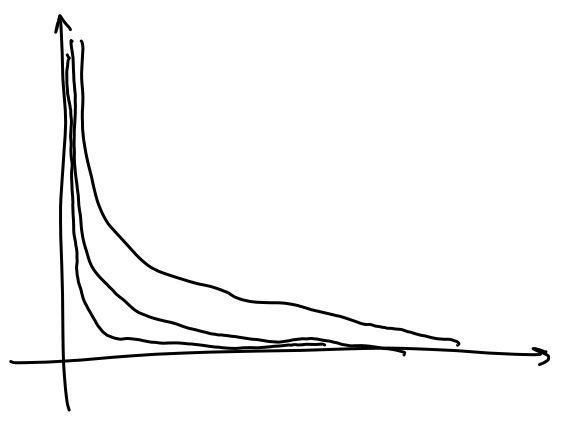
\includegraphics[scale=0.3]{2_2.png}
\end{center}
\(f_n(x) = \frac{1}{nx}, x > 0\) \\
\(X \ \R_+\ \lambda\) \\
\(f_n \to f\) всюду на \((0, + \infty)\) \\
\(f_n \xRightarrow[\lambda]{} f\)
\end{examp}
\begin{examp}
\-
\begin{center}
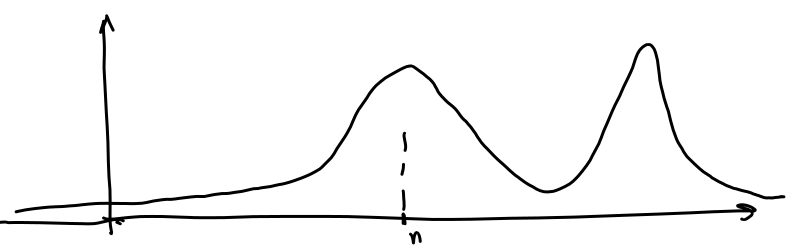
\includegraphics[scale=0.3]{2_3.png}
\end{center}
\(f_n(x) := e^{-(n - x)^2}\ x \in \R\) \\
\(f_n(x) \to 0\) при всех \(x\) \\
\(f_n(x) \rightarrow 0\) \\
\[ \mu (\R(e^{-(n - x)^2} \ge \varepsilon)) = \const \not\to 0 \]
, при \(0 < \varepsilon < 1\)
\end{examp}
\begin{examp}
\(n = 2^k + e, 0 \le e < 2^k\) \\
\(X = [0, 1]\ \lambda\) \\
\(f_n(x) := \X_{[\frac{e}{2^k}, \frac{e + 1}{2^k}]}\) \\
\(\lim f_n(x)\) --- не существует ни при каких \(x\) \\
\[ \lambda X(f_n > \varepsilon) = \frac{1}{2^k} \xrightarrow[n \to + \infty]{} 0 \]
\[ f_n \xRightarrow[\lambda]{} 0 \]
\end{examp}
\begin{theorem}[Лебега]
\-
\begin{itemize}
\item \((X, \A, \mu)\)
\item \(f_n, f\) --- измеримые, почти везде конечные
\item \(f_n \to f\) почти везде
\item \(\mu X\) --- конечна
\end{itemize}
\uline{Тогда} \(f_n \xRightarrow[\mu]{} f\)
\end{theorem}
\begin{proof}
Переопределим \(f_n, f\) на множестве меры 0, чтобы сходимость была всюду
\uline{Частный случай}: \(\forall x\) последовательность \(f_n(x)\) монотонно убывает к 0(т.е. \(f < 0\))
\[ \left.\begin{array}{cc}X(|f_n| \ge \varepsilon) = X(f_n \ge \varepsilon) \supset X(f_{n + 1} \ge \varepsilon) \\ \bigcap X(f_n \ge \varepsilon) = \emptyset \end{array}\right\} \Rightarrow \text{Теорема о непрерывность меры сверху}\]
\uline{Общий случай}: \(f_n \to f\)
\[ \varphi_n(x) = \sup_{k \ge n}|f_k(x) - f(x)| \]
Тогда \(\varphi_n \to 0\), монотонна
\[ X(|f_n - f| \ge \varepsilon) \subset X(\varphi_n \ge \varepsilon) \]
\[ \mu X(|f_n - f| \ge \varepsilon) \le \mu X(\varphi_n \ge \varepsilon) \to 0 \]
\end{proof}
\begin{theorem}[Рисс]
\-
\begin{itemize}
\item \((X, \A, \mu)\)
\item \(f_n, f\) --- измеримы почти везде, конечны
\item \(f_n \xRightarrow[\mu]{} f\)
\end{itemize}
\uline{Тогда} \(\exists n_k f_{n_k} \to f\) почти везде
\end{theorem}
\begin{proof}
\(\forall k\ \mu X(|f_n - f| \ge \frac{1}{k}) \to 0\) \\
\(\exists n_k\): при \(n > n_k\ \mu X(|f_n - f| \ge \frac{1}{k}) < \frac{1}{2^k}\) \\
можно считать: \(n_1 < n_2 < n_3\) \\
Проверим \(f_{n_k} \to f\) почти везде
\[ E_k := \bigcup_{i = k}^{+ \infty} X(|f_{n_i} - f| \ge \frac{1}{i})\quad E = \bigcap E_i \]
\[ E_k \supset E_{k + 1}\quad \mu E_k \le \sum_{i = k}^{+ \infty}\mu X(|f_{n_i} - f| \ge \frac{1}{i}) < \sum_{i = k}^{+ \infty}\frac{1}{2^i} \le \frac{2}{2^k} \to 0 \]
\[ \mu E_k \to \mu E \Rightarrow \mu E = 0 \]
При \(x \not\in E\ f_{n_k} \to f\) \\
\[ x\not\in E\ \exists N\ x\not\in E_k$ при $k > N \quad |f_{n_k}(x) - f(x)| < \frac{1}{k} \]
, т.е. \(f_{n_k}(x) \to f(x)\)
\end{proof}
\begin{corollary}
\-
\begin{itemize}
\item \(f_n \xRightarrow[\mu]{} f\)
\item \(|f_n| \le g\) почти везде
\end{itemize}
\uline{Тогда} \(|f| \le g\) почти везде
\end{corollary}
\begin{proof}
\(\exists n_k:\ f_{n_k} \to f\) почти везде
\end{proof}
\begin{theorem}[Егорова]
\-
\begin{itemize}
\item \(\mu X < + \infty\)
\item \(f_n, f\) --- почти везде конечны, измеримы
\item \(f_n \to f\) почти везде
\end{itemize}
\uline{Тогда}  \(\forall \varepsilon > 0\ \exists e \subset X,\ \mu e < \varepsilon\quad f_n \rightrightarrows f\) на \(X \setminus e\)
\end{theorem}
\xymatrix@1{A\ar[r]^>>{+}&B}

\section{Интеграл}
\label{sec:org156492e}
\((X, \A, \mu)\)
\begin{definition}
\label{def_int_1}
\(f = \sum \alpha_k \X_{E_k}\quad\begin{array}{c} E_k\text{ --- дополнительное разбиение} \\ \alpha_k \ge 0 \end{array}\) \\
\[ \int_X f d\mu = \sum \alpha_k \mu E_k \]
, считаем \(0\cdot + \infty = 0\)
\end{definition}
\begin{remark}
Свойства:
\begin{enumerate}
\item Не зависит от представления \(f\) в виде сумме \\
\[ f = \sum \alpha_k \X_{E_k} = \sum \alpha'_k\X_{E'_k} = \sum_{k,j}\alpha_k \X_{E_k\cap E'_j} \]
\[ \int f = \sum \alpha_k \mu E_k \]
\item \(f \le g\quad\int f \le \int g\), \(f, g\) --- ст.
\end{enumerate}
\end{remark}
\begin{definition}
\label{def_int_2}
\(f \ge 0\) --- измерима \\
\[ \int_X f d\mu := \sup_{\substack{g\text{ --- ступ.} \\ 0 \le g \le f}} \int g d\mu \]
\end{definition}
\begin{remark}
Свойства:
\begin{enumerate}
\item Если \(f\) --- ступенчатая то \hyperref[def_int_1]{Опр. 2} = \hyperref[def_int_2]{Опр. 1}
\item \(0 \le \int f \le + \infty\)
\item \(g \le f\), \(f\) --- измерима, \(g\) --- ступенчатая \(\Rightarrow\) \(\int_X g \le \int_X f\)
\end{enumerate}
\end{remark}
\begin{definition}
\-
\begin{itemize}
\item \(f\) --- измерима
\item \(\int_X f^+\) или \(\int_x f^-\) конечный
\end{itemize}
\uline{Тогда} \[ \int_X f d\mu = \int_X f^+ d\mu - \int_X f^- d\mu \]
\end{definition}
\begin{theorem}[Тонедди]
\-
\begin{itemize}
\item \(f: \R^{m + n} \to \overline{\R}\)
\item \(f \ge 0\) --- измерима
\item \(E \subset \R^{m + n}\)
\end{itemize}
\begin{symb}
\(\forall x \in \R^m\quad E_x = \{ y\in\R^n : (x, y) \in E\}\)
\end{symb}
\uline{Тогда}
\begin{center}
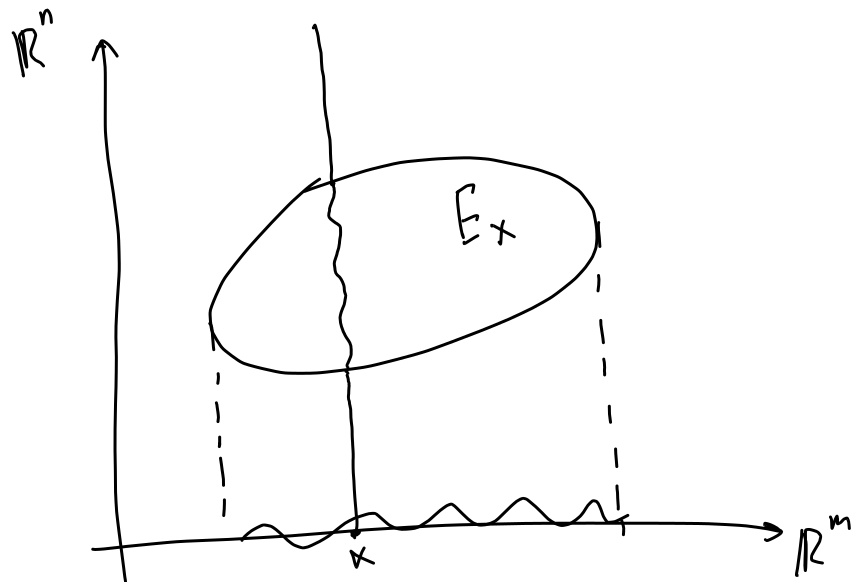
\includegraphics[scale=0.3]{2_4.png}
\end{center}
\begin{enumerate}
\item при почти всех \(x \in \R^m\) функция \(y\mapsto f(x, y)\) --- измерима на \(\R^n\)
\item функция \[ x \mapsto \int_{E_k} f(x, y) d\lambda_n(y) \ge 0 \]
\item \[ \int_E f(x, y) d\mu = \int_{\R^m}\left(\int_{E_x} f(x, y d\lambda_n(y))\right)d\lambda_m(x) \]
\end{enumerate}
\end{theorem}
\chapter{}
\label{sec:org28dbc18}
\newcommand{\X}{\mathcal{X}}
\newcommand{\A}{\mathfrak{A}}

\section{Интеграл}
\label{sec:orgd64f09c}
\begin{enumerate}
\item \(f \ge 0\), ступенчатые \\
\(f = \sum_\text{кон.} \alpha_k \chi_{E_k}\), \(E_k\) --- измеримое \\
\(\int_X f = \sum \alpha_k \mu E_k\)
\item \label{int_3_2} \(f \ge 0\), измеримая \\
\(\int_X f d\mu = \sup_{\substack{0 \le g \le g \\ f\text{ --- ступ.}}} \int_X g d\mu\)
\item \label{int_3_3} \(f\) --- измерима, \(f^+, f^- \ge 0\) --- измеримые \\
Пусть \(\int_X f^+\) или \(\int_X f^-\) --- конечные \\
Тогда \(\int_X f = \int_X f^+ - \int_X f^-\)
\begin{definition}
Если \(\int_x f^+,\ \int_X f^-\) --- оба конечные, то \(f\) назывется \textbf{суммируемой}
\end{definition}
\begin{remark}
\(f\) --- измеримая, \(\ge 0\), интеграл \ref{int_3_3} = интеграл \ref{int_3_2}
\end{remark}
\item \begin{definition}
\(E \subset X\) --- измкримое, \(f\) --- измерима на \(X\) \\
\(\int_E f d\mu = \int_X f\cdot\chi_E\)
\end{definition}
\end{enumerate}

\begin{remark}
\(f = \sum \alpha_k \chi_{E_k}\ \int_E f = \sum \alpha_k \mu(E_k \cap E)\)
\end{remark}
\begin{remark}
\(\int_E f d\mu = \sup \{fg:\ 0 \le g \le f\text{ на } E, g\text{ --- ступенчатые}\}\), можно считать что \(g\) ---
тождественный 0 вне множества \(E\)
\end{remark}
\begin{remark}
\(\int_E f\) не зависит от значений \(f\) вне \(E\)
\end{remark}
\begin{remark}
\((X, \A, \mu)\) \(E\subset X\) --- измеримое, \(g, f\) --- измеримые. Свойства:
\begin{enumerate}
\item \label{prop_3_1} Монотонность \(f \le g\) \(\int_E f \le \int_E g\)
\begin{proof}
\-
\begin{center}
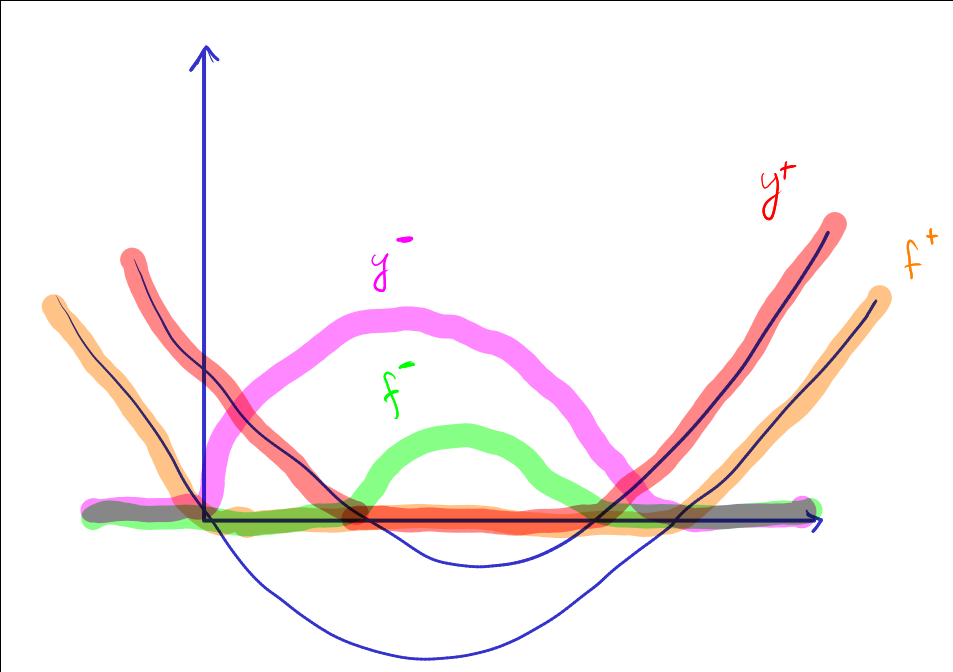
\includegraphics[scale=0.3]{3_1.png}
\end{center}
\begin{enumerate}
\item \(f, g \ge 0\) --- очевидно
\item \(f, g\) --- произвольные \\
\(f^+ \le g^+\ f^- \le g^-\) \\
\(\int_E f^+ \le \int_E g^+\ \int_E f^- \le \int_E g^- \Rightarrow \text{OK}\)
\end{enumerate}
\end{proof}
\item \(\int_E Ad\mu = \mu E\ \int_E 0 d\mu = 0\)
\item \label{prop_3_3} \(\mu E = 0\ \int_E f= 0\)
\begin{proof}
\begin{enumerate}
\item \(f\) --- ступенчатая
\item \(f \ge 0\) --- измеримая
\end{enumerate}
\end{proof}

\emph{Змечание}: \\
\(f\) --- измеримая. Тогда \(f\) --- суммируемая \(\Leftrightarrow\) \(\int |f| < + \infty\) \\
\begin{description}
\item[{\((\Leftarrow)\)}] следует из cвойства \ref{prop_3_1}. \(f^+, f^- \le |f|\)
\item[{\((\Rightarrow)\label{remark_3_1_proof}\)}] позже
\end{description}
\item \label{prop_3_4} \(\int_E(-f) = -\int_E f,\ \forall c \in \R\ \int_E c f = c\int_E f\) \\
\begin{enumerate}
\item \((-f)^+ = f^-\ (-f)^- = f^+\)
\item можно считать \(c > 0\) для \(f \ge 0\) --- тривиально
\end{enumerate}
\item \(\exists \int_E f d\mu\) \\
Тогда \(|\int_E f d\mu| \le \int_E |f| d\mu\)
\begin{proof}
\(-|f| \le f \le |f|\). По свойствам \ref{prop_3_3} и \ref{prop_3_4}
\end{proof}
\item \(\mu E \le +\infty,\ a\le f\le b\) \\
Тогда \(a\mu E \le \int_E f \le b \mu E\)
\(\color{gray} a\chi_E \le f \le b\chi_E\)
\begin{corollary}
\(f\) --- измерима на \(E\), \(f\) --- ограничена на \(E\), \(\mu E < + \infty\) \\
Тогда \(f\) --- суммируемая на \(E\)
\end{corollary}
\item \(f\) --- суммируемая на \(E\). Тогда \(f\) --- почти везде конечная
\begin{proof}
\-
\begin{enumerate}
\item \(f \ge 0\ f = + \infty\) на \(A \subset E\) \(\forall n \in \N\ \int_E f \ge n\mu A\)
\item \(f = f^+ - f^-\)
\end{enumerate}
\end{proof}
\end{enumerate}
\end{remark}
\begin{lemma}
\label{lemma_3_1}
\[ A = \bigsqcup_{i - 1}^{ + \infty} A_i \]
--- измеримые, \(g\) --- ступенчатая, \(g \ge 0\) \\
\uline{Тогда} \[ \int_A g d\mu = \sum_{i = 1}^{ + \infty}\int_{A_i}g d\mu \]
\end{lemma}
\begin{proof}
\(\int_A g d\mu = \sum_\text{кон.} \alpha_k \mu(E_k \cap A) = \sum_k\sum_i \underbrace{\alpha_k\mu(E_k \cap A_i)}_{\ge 0} = \sum_i \sum_k \dots = \sum_i\int_{A_i} gd\mu\)
\end{proof}
\begin{theorem}
\(A = \bigsqcup A_i\) --- измеримые, \(f: X \to \overline{\R}\) --- измеримая на \(A\), \(f \ge 0\) \\
\uline{Тогда} \(\int_A fd\mu = \sum_{i = 1}^{ + \infty} \int_{A_i} f d\mu\)
\end{theorem}
\begin{proof}
\-
\begin{description}
\item[{\((\le)\)}] ступенчатая \(g:\ 0 \le g \le f\ \int_a g = \sum\int_{A_i} g d\mu \le \sum \int_{A_i} f\) --- по \hyperref[lemma_3_1]{Лемме}
\item[{\((\ge)\)}] \begin{enumerate}
\item \(A = A_1 \cup A_2\) \\
\(0 \le g_1 \le f\chi_{A_1}\ 0 \le g_2 \le f\chi_A_2}\) \\
\[ g_1 = \sum \alpha_k \chi_{E_k}\ g_2 = \sum \beta_k \chi_{E_k} \]
\begin{center}
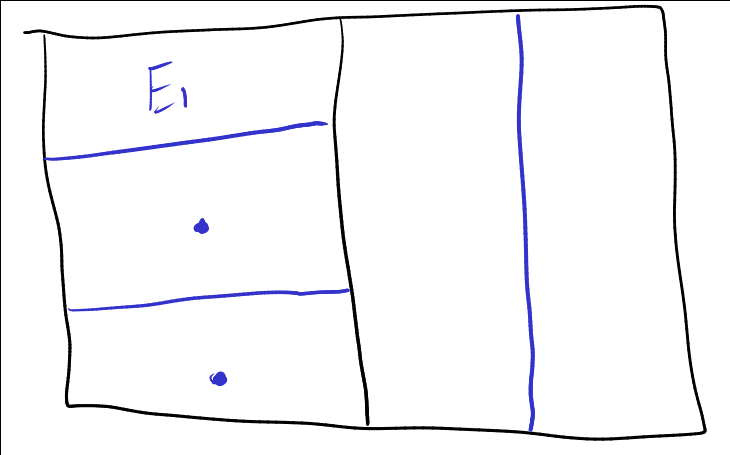
\includegraphics[scale=0.3]{3_2.png}
\end{center}
Считаем что \(E_k\) -- совместное разбиение
\[ 0 \le g_1 + g_2 \le f \chi_A \]
\[ \int_{A_1} g_1 + \int_{A_2} g_2 =  \int_A g_1 + g_2 \le \int_A f \]
Перейдем к супремуму
\[ \int_{A_1} f + \int_{A_2} g_2 \le \int_A f \]
\[ \int_{A_1} f + \int_{A_2} f \le \int_A f \]
\item \(\forall n \in \N\) --- индукция по \(n\)
\item \[ A = \bigsqcup_{i = 1}^n A_i \sqcup B_n \], где \[ B_n = \bigsqcup_{i > n} A_i \]
\[ \int_A f = \sum_{i = 1}^n \int_{A_i} f + \int_{B_n} f \ge \sum_{i = 1}^n \int_{A_i} f \]
\end{enumerate}
\end{description}
\end{proof}
\begin{corollary}
\begin{itemize}
\item \(f \ge 0\) --- измеримая
\item \(\nu: \A \to \overline{\R}_+\)
\item \(\nu E := \int_E fd\mu\)
\end{itemize}
\uline{Тогда} \(\nu\) --- мера
\end{corollary}
\begin{corollary}[аддитивности интеграла]
\(f\) --- суммируема на \(A = \bigsqcup A_i\) --- измеримые \\
\uline{Тогда} \[ \int_A f = \sum \int_{A_i} f \]
\end{corollary}
\begin{proof}
\(f^+, f^- \dots\) \(\color{red}???\)
\end{proof}
\subsection{Предельный переход под щнаком интеграла}
\label{sec:org2fc001a}
\(f_n \to f\). Можно ли утверждать \(\int_E f_n \to \int_E f\)?
\begin{examp}
\(f_n, f: \R \to \R\) \\
\(f_n = \frac{1}{n} \cdot \chi_{[0, n]}\ f\equiv 0\ f_n \to f\) (даже \(f_n \rightrightarrows f\) на \(\R\)) \\
\[ \int_\R f_n = \frac{1}{n}\lambda[0, n] = 1\not \xrightarrow[n \to + \infty]{} 0 = \int_\R f \]
\end{examp}
\begin{theorem}[Леви]
\((X, \A, \mu)\), \(f_n\) --- измеримая \\
\(\forall n\ 0 \le f_n \le f_{n + 1}\)  почти везде \(f(x) := \lim_{n\to + \infty} f_n(x)\) почти везде \\
\uline{Тогда} \(\lim_{n \to + \infty}\int_X f_n d \mu = \int_x fd\mu\)
\end{theorem}
\begin{remark}
\(f\) --- задана всюду, кроме множества меры \(0\). Считаем, что \(f = 0\) на \(e\) \\
\uline{Тогда} \(f\) --- измерима на \(X\).
\end{remark}
\begin{proof}
\-
\begin{description}
\item[{\((\le)\)}] очевидно. \(f_n \le f\) почти везде \(\int f_n \le \int f\)
\[ \int_X f_n = \int_{X\setminus e}f_n + \int_e f_n = \int_{X\setminus e} f_n \le \int_{X \setminus e} f \le \int_X f \]
\item[{\((\ge)\)}] Достаточно: \(\forall g\) --- ступенчатая \(0 \le g \le f\)
\[ \lim \int_X f_n \ge \int_X g \]
Достаточно: \(\forall c \in (0, 1)\)
\[ \lim \int_X f_n \ge c \int_X g \]
\[ E_n := X(f_n \le c g) \dots \subset E_n \subset E_{n + 1} \subset \dots \]
\(\bigcup E = X\) т.к. \(c < 1\)
\[ \int_x f_n \ge \int_{E_n} f_n \ge c \int_{E_n} g \]
Тогда \(\lim \int_X f_n \ge c \lim \int_{E_n} g = c\int_X g\) \\
Последнее равентсво справедливо в силу непрерывности мнизу меры \(\nu: E \mapsto \int_E g\)
\end{description}
\end{proof}

\begin{theorem}
\(f, g \ge 0\) измерима на \(E\) \\
\uline{Тогда} \[ \int_E f + g = \int_E f + \int_E g \]
\end{theorem}
\begin{proof}
\-
\begin{enumerate}
\item \(f, g\) --- ступенчатые \\
\[ f = \sum \alpha_k\chi_{E_k},\ g = \sum \beta_k\chi_{E_k} \]
\[ \int_E f + g = \sum (\alpha_k + \beta_k)\mu(E_k \cap E) = \sum \alpha_k \mu(E_k \cap E) + \sum \beta_l \mu(E_k \cap E) = \int_E f + \int_E g \]
\item \(f \ge 0\) --- измерима \(\Rightarrow\) \(\exists\) стпенчатая \(f_n:\ 0 \le f_n \le f_{n + 1} \le \dots \ \lim f_n = f\) \\
\(g \ge 0\) --- измерима \(\Rightarrow\) \(\exists\) стпенчатая \(g_n:\ 0 \le g_n \le g_{n + 1} \le \dots \ \lim g_n = g\) \\
\(f_n + g_n \to f + g\ \int_E f_n + g_n \to \int_E f + g\) \\
\(\int_E f_n + g_n = \int_E f_n + \int_E g_n \to \int_E f + \int_E g = \int_E f+g\)
\end{enumerate}
\end{proof}
\begin{corollary}
\(f, g\) --- суммируемы на \(E\) \\
\uline{Тогда} \(f+g\) --- суммируема и \(\int_E f + g = \int_E f + \int_E g\)
\end{corollary}
\begin{remark}
Свойство \(\ref{remark_3_1_proof}\) доказано
\end{remark}
\begin{proof}
Суммируемость \(|f+g|\le |f| + |g|\) \\
\(h = f + g\). Тогда:
\[ h^+ - h^- = f^+ - f^- + g^+ - g^- \Leftrightarrow h^+ + f^- + g^- = h^- + f^+ + g^+ \]
\[ \Rightarrow \int_E h^+ + \int_E f^- + \int_E g^- = \int_E h^- + \int_E f^+ + \int_E g^+ \]
\[ \int_E h^+ - \int_E h^- = \int_E f^+ - \int_E f^- + \int_E g^+ - \int_E g^- \]
\[ \int_E h = \int_E f + \int_E g \]
\end{proof}
\begin{definition}
\(\mathcal{L}(X) =\) множество функций суммируемых на X
\end{definition}
\begin{corollary}
\(\mathcal{L}(X)\) --- линейное пространство, а отображение \(f \mapsto \int_X f\) --- это линейный функционал на \(\mathcal{L}(X)\)
, т.е. \(\forall f_1, \dots, f_n \in \mathcal{L}(X)\ \forall \alpha_1, \dots, \alpha_k \in \R\)
\[ \sum_{k = 1}^n \alpha_k f_k \in \mathcal{L}(X);\ \int_X\sum\alpha_k f_k = \sum_{k = 1}^n\alpha_k\int_X f_k\]
\end{corollary}
\begin{theorem}[об интегрировании положительных рядов]
\((X, \A, \mu)\ E \in \A\ \underset{\text{изм.}}{u_n}: X \to \overline{\R}\ u_n \ge 0\) почти везде \\
\uline{Тогда} \[ \int_E(\sum_{n = 1}^{ + \infty} u_n(x))d\mu(x) = \sum_{n = 1}^{ + \infty} \int_E u_n d\mu \]
\end{theorem}
\begin{proof}
по т. Леви: \(S_n := \sum_{k = 1}^n u_k\ 0 \le S_n \le S_{n + 1} \le \dots\ S_n \to S\) --- сумма ряда \(\sum u_n\) \\
Тогда \(\int_E S_n \to \int_E S\), \(\int_E S_n = \sum_{k = 1}^n \int_E u_k \to \int_E S\)
\end{proof}
\begin{corollary}
\(u_n\) --- измеримые \(\sum_{n = 1}^{ + \infty} \int_E |u_n| < + \infty\) \\
\uline{Тогда} ряд \(\sum u_n(x)\) --- абсолютно сходится при почти всех \(x\)
\end{corollary}
\begin{proof}
\(S(x) := \sum |u_n(x)| \ge 0\) --- измеримая
\[ \int_E S(x) = \sum \int_E |u_n| < + \infty \]
\(\Rightarrow\) \(S\) --- сумиируема \(\Rightarrow\) \(S\) почти везде конечена
\end{proof}
\begin{examp}
\(x_n \in \R\) --- произведение последовательности; \(\sum a_n\) --- абсолютно сходится \\
\uline{Тогда} \(\sum \frac{a_n}{\sqrt{|x - x_n|}}\) --- абсолютно сходится при почти всех \(x\)
\end{examp}
\begin{proof}
Достаточно проверить абсолютную сходимость на \([-N, N]\) почти везде
\begin{center}
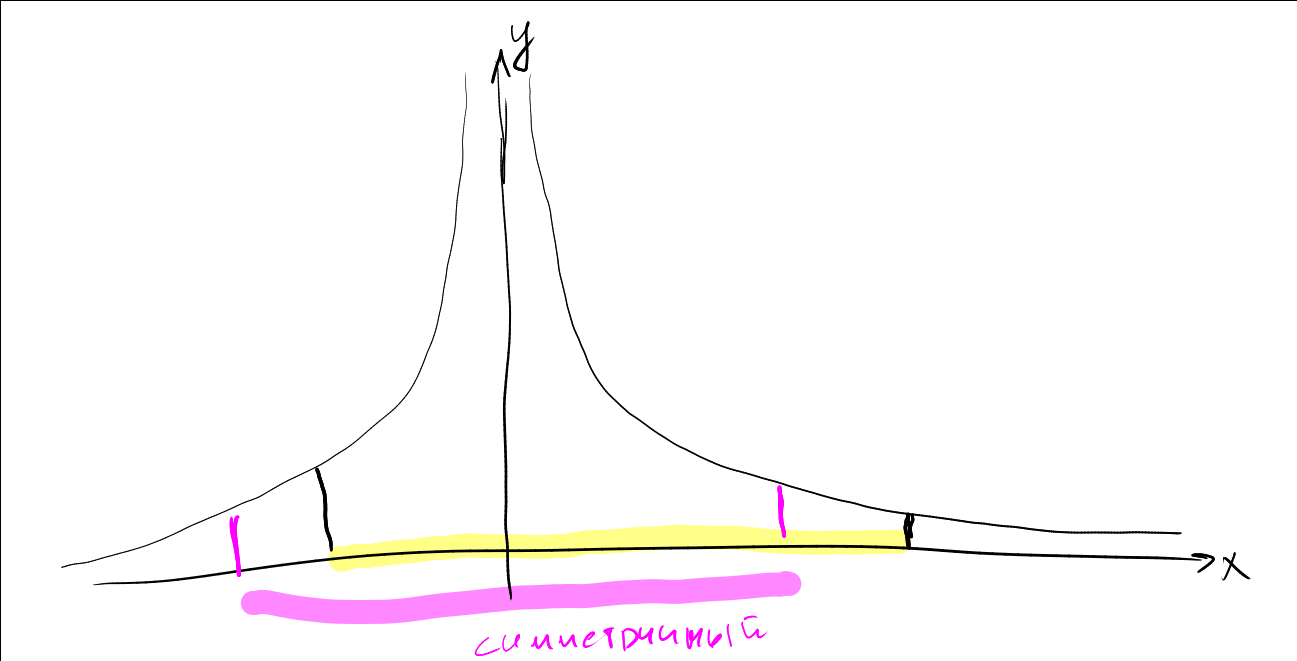
\includegraphics[scale=0.3]{3_3.png}
\end{center}
\[ \int_{[-N , N]} \frac{|a_n|}{\sqrt{|x - x_n|}} = \int_{-N}^N \frac{|a_n|}{\sqrt{|x - x_n|}} dx = |a_n| \int_{-N - x_n}^{N - x_n} \frac{dx}{\sqrt{|x|}} \le \]
\[ \le |a_n| \int_{-N}^N \frac{dx}{\sqrt{|x|}} = 4\sqrt{N}\cdot|a_n| \]
\[ \sum_n \int_{[-N, N]}\frac{|a_n|}{\sqrt{|x - x_n|}} \le 4 \int_N \sum |a_n| < + \infty \]
\end{proof}
\chapter{}
\label{sec:orgdb0785a}
\newcommand{\X}{\mathcal{X}}
\newcommand{\A}{\mathfrak{A}}
\newcommand{\B}{\mathfrak{B}}

\begin{theorem}[об абсолютной непрерывности ингтерала]
\-
\begin{itemize}
\item \((X, \A, \mu)\)
\item \(f: X \to \overline{\R}\) --- суммируема
\end{itemize}
\uline{Тогда} \(\forall \varepsilon > 0\ \exists \delta > 0\ \forall E\) --- измеримым, \(\mu E < \delta\quad |\int_E f| < \varepsilon\)
\end{theorem}
\begin{corollary}
\-
\begin{itemize}
\item \(f\) --- суммируемая
\item \(\mu E \to 0\)
\end{itemize}
\uline{Тогда} \(\int_{E_n} f \to 0\)
\end{corollary}
\begin{proof}
Возьмем множества \(X_m := X(|f| \ge n)\), очевидно что \(X_n \supset X_{n + 1} \supset \dots\), а также \(\mu(\bigcap X_n) = 0\) \\
Утвержение: \(\forall \varepsilon\ \exists n_\varepsilon\quad \int_{X_{n_\varepsilon}}|f| < \frac{\varepsilon}{2}\) ---
это свойство непрерывности сверху меры \(A \mapsto \int_A |F| d\mu\) \\
Пусть \(\delta:=\frac{\varepsilon}{2n_\varepsilon}\), тода при \(\mu E < \delta\)
\[ \left|\int_E f\right| \le\int_{E_nX_{n_\varepsilon}}|f| + \int_{E_nX_{n_\varepsilon}}^C \le \int_{X_{n_\varepsilon}} |f| + \int_{E_nX_{n_\varepsilon}} n_\varepsilon < \frac{\varepsilon}{2} + \mu E\cdot n_\varepsilon \le \varepsilon \]
\end{proof}
Правда ли что:
\[ f_n \xRightarrow[\mu]{} f\quad \forall \varepsilon > 0\ \mu X(|f_n - f| > \varepsilon) \to 0\]
\[ \int_X|f_n - f| d\mu \to 0 \]
эквивалентны.
\begin{description}
\item[{\((\Rightarrow)\)}] \textbf{Нет}. \((X, \A, \mu) = (\R, \mathfrak{M}, \lambda)\) \\
\(f_n = \frac{1}{nx}\ f_n \xRightarrow[\lambda]{} 0\) \\
\(\int|f_n - f| = + \infty\) --- при всех \(n\)
\item[{\((\Leftarrow)\)}] \textbf{Да}. \[\mu \underbrace{X(|f_n - f| > \varepsilon)}_{X_n} = \int_{X_n} 1 \le \int_{X_n} \frac{|f_n - 1|}{\varepsilon} = \frac{1}{\varepsilon}\int_{X_n}|f_n - f| \le \frac{1}{\varepsilon}\int_X|f_n - f| \xrightarrow[n\to +\infty]{} 0\]
\end{description}
\begin{theorem}[Лебега]
\-
\begin{itemize}
\item \((X, \A, \mu)\)
\item \(f_n, f\) --- измеримые, почти везде конечные
\item \(f_n \xRightarrow[\mu]{} f\)
\item \(\exists g\) --- \textbf{суммируемая мажоранта}:
\begin{enumerate}
\item \label{lebega_1} \(\forall n\ |f_n| \le g\) почти везде
\item \(g\) --- усммируемая везде
\end{enumerate}
\end{itemize}
\uline{Тогда} \(f_n, f\) --- суммируемые и \(\int_X |f_n - f|d\mu\xrightarrow[n \to + \infty]{}0\), и 'тем более' \(\int_X f_n d\mu \to \int_X f d\mu\)
\end{theorem}
\begin{proof}
\(f_n\) --- суммируема в силу \ref{lebega_1}, \(f\) --- суммируема по следствию т. Рисса: \(|f| \le g\) почти везде \\
'тем более' = \(\left|\int_X f_n - \int_X f \right| \le \int_X |f_n - f| \to 0\)
\begin{enumerate}
\item \label{lebega_2} \(\mu X < + \infty\) фиксируем \(\varepsilon\ X_n = X(|f_n - f| > \varepsilon)\) \\
\(f_n \to f\), т.е. \(\mu X_n \to 0\)
\[ |f_n - f| \le |f_n| + |f| \le 2g \]
\[ \int_X|f_n - f| = \int_{X_n}+\int_{X_n^C} \le \int_{X_n} 2g + \int_{X_n^C} \varepsilon d\mu < \varepsilon + \varepsilon \mu X\]
По следствию т. об абсолютной непрерывности: \(\int_{X_n} 2g \xrightarrow[n \to + \infty]{} 0\)
\item \(\mu X = + \infty\) \\
Проверим утверждение: \(\forall \varepsilon > 0\ \exists A \subset X\) --- измеримое, \(\mu A\) --- конечная: \(\int_{X\setminus A} g < \varepsilon\)
\[ \int_X g = \sup \{\int g_n,\ 0\le g_n\le g,\ g_n\text{ --- ступенчатая}\} \]
\[ A := \{x:\ g_n(x) > 0\} \]
--- при достаточно больших \(n\)
\[\color{blue} 0 \le \int_X g - \int_X g_n = \int_A g- g_n + \int_{X\setminus A}g < \varepsilon \]
Фиксируем \(\varepsilon > 0\)
\[ \int_X |f_n - f| d\mu = \int_A + \int_{X\setminus A} \le \int_A |f_n -f| + \int_{X\setminus A}2g \]
По \ref{lebega_2} \(\int_A|f_n - f| \xrightarrow[n \to + \infty]{} 0\ \int_{X\setminus A}2g < 2\varepsilon\) \\
т.е. при больших \(n\) \(\int_x |f_n -f|d\mu < 2\varepsilon\)
\end{enumerate}
\end{proof}

\begin{theorem}[Лебега]
\-
\begin{itemize}
\item \((X, \A, \mu)\)
\item \(f_n, f\) --- измеримые, почти везде конечные
\item \(f_n \to f\) почти везде
\item \(\exists g\) --- \textbf{суммируемая мажоранта}:
\begin{enumerate}
\item \label{lebega_1} \(\forall n\ |f_n| \le g\) почти везде
\item \(g\) --- усммируемая везде
\end{enumerate}
\end{itemize}
\uline{Тогда} \(f_n, f\) --- суммируемые и \(\int_X |f_n - f|d\mu\xrightarrow[n \to + \infty]{}0\), и 'тем более' \(\int_X f_n d\mu \to \int_X f d\mu\)
\end{theorem}
\begin{proof}
\[ h_n := \sup(|f_n - f|,\ |f_{n + 1} - f|,\ \dots) \]
\begin{itemize}
\item \(0 \le h_n \le 2g\)
\item \(h_n\) --- монотонна убывает
\item \(\lim h_n = \overline{\lim}|f_n - f| = 0\) почти везде
\end{itemize}
\(2h - h_n \ge 0\) --- эта последовательность возрастает, \(2g - h_n \to 2g\) почти везде
\[ \int_X 2g - h_n \to \int_X 2g \Rightarrow \int_X h_n \to 0 \]
\[ \int_X|f_n -f| \le \int_X h_n \to 0 \]
\end{proof}
\begin{examp}
\[ \int_0^{ + \infty} t^{x - 1}e^{-t} dt \]
\[ \lim_{x \to x_0} \int_0^{ + \infty} t^{x - 1} e^{-t} dt \overset{?}{=} \int_0^{ + \infty}t^{x_0 - 1}e^{-t} dt\]
\textbf{Да}. \(t^{x - 1} e^{-t} \xrightarrow[x \to x_0]{} t^{x_0 - 1}e^{-t}\) при всех \(t>0\) \\
Суммируемая мажоранта: \(|t^{x - 1}e^{-t}| \le \underbrace{t^{\alpha - 1}e^{-t}}_\text{сумм.}\), \(0 < \alpha < x_0\)
\end{examp}

\begin{theorem}[Фату]
\begin{itemize}
\item \((X, \A, \mu)\)
\item \(f_n \ge 0\) --- измеримая
\item \(f_n \to f\) почти везде
\item \(\exist c > 0\ \forall n\ \int_X f_n \le c\)
\end{itemize}
\uline{Тогда} \(\int_X f \le c\) \\
\end{theorem}
\begin{remark}
Здесь не требуется чтобы \(\int_X f_n \to \int_X f\), это может быть не выполнено
\end{remark}
\begin{proof}
\[ g_n := \inf(f_n,\ f_{n + 1},\ \dots) \]
\[ 0 \le g_n \le g_{n + 1}\ \lim g_n = \underline{\lim} f_n = f\text{ почти везде} \]
\[ \int_X g_n \le \int_X f_n \le c \]
\[ \int_X g_n \to \int_X f \Rightarrow \int_X f \le c \]
\end{proof}
\begin{corollary}
\-
\begin{itemize}
\item \(f_n, f \ge 0\) --- измеримые, почти везде конечные
\item \(f_n \Rightarrow f\)
\item \(\exists c >0\ \forall n \int_X f_n \le c\)
\end{itemize}
\uline{Тогда} \(\int_X f \le c\)
\end{corollary}
\begin{proof}
\[ f_n \Rightarrow f \Rightarrow \exists n_k\ f_{n_k} \to f\text{ почти везде} \]
\end{proof}

\begin{corollary}
\-
\begin{itemize}
\item \(f_n \ge 0\) --- измеримые
\end{itemize}
\uline{Тогда} \[ \int_X \underline{\lim}f_n \le \underline{\lim}\int_X f_n \]
\end{corollary}
\begin{proof}
Как в теореме: \[ \int_X g_n \le \int_X f_n \]
Выберем \(n_k\): \[ \int_X f_{n_k} \xrightarrow[n \to + \infty]{} \underline{\lim}\int_X f_n \]
\color{red}Zzz..\color{black}
\end{proof}
\section{Плотность одной меры по отношению к другой}
\label{sec:org1505d20}
\subsection{Замена перменных в интеграле}
\label{sec:org63e16a8}
\begin{itemize}
\item \((X, \A, mu)\)
\item \((Y, \B, \cdot)\)
\item \(\Phi: X \to Y\)
\end{itemize}


\begin{itemize}
\item Пусть \(\Phi\) --- измеримо в следующем смысле:
\[ \Phi^{-1}(\B) \subset \A \]
\end{itemize}

\noindentДля \(E \in \B\) положим \(\nu(E) = \mu \Phi^{-1}(E)\) \\
Тогда \(\nu\) --- мера:
\[ \nu(\bigsqcuo E_n) = \mu(\Phi^{-1}(\bigsqcup E)n) = \mu(\bigsqcup\Phi^{-1}(E_n)) = \sum \mu \Phi^{-1} (E_n) = \sum \nu E_n\]
Мера \(\nu\) называется образом \(\mu\) при отображении \(\Phi\) и
\[ \nu E = \int_{\Phi^{-1}(E)} 1 d\mu \]
\begin{remark}
\-
\begin{itemize}
\item \(f: Y \to \overline{\R}\) --- измерима относительно \(\B\)
\end{itemize}
Тогда \(f\circ \Phi\) --- измерима относитльно \(\A\ (f\circ \Phi: X\to\overline{\R})\)
\[ X(f(\Phi(x)) < a) = \Phi^{-1}(\underbrace{Y(f < a)}_{\in \B}) \in \A \]
\end{remark}

\begin{definition}
\-
\begin{itemize}
\item \(\omega: X\to\overline{\R}\) --- измерима(на \(X\) относительно \(\A\))
\item \(\omega \ge 0\)
\end{itemize}
\[ \forall B \in \B\ \nu(B) = \int_{\Phi^{-1}(B)}\omega(x)d\mu(x) \]
--- \textbf{взвешенный образ меры} \(\mu\) при отображении \(\Phi\), \(\omega\) --- \textbf{вес}
\end{definition}
\begin{theorem}
\-
\begin{itemize}
\item \((X, \A, \mu)\)
\item \((Y, \B, \nu)\)
\item \(\Phi: X \to Y\)
\item \(\nu\) --- взвешенный образ меры \(\mu\) при отображении \(\Phi\) с весом \(\omega\)
\item \(\omega \ge 0\) --- измерима на \(X\)
\end{itemize}
\uline{Тогда} \(\forall f\) --- измеримые на \(Y\) относительно \(\B\), \(f \ge 0\) \(f\circ \Phi\) --- измеримая на \(X\) относительно \(\A\) и
\[ \int_Y f(y) d\nu(y) = \int_X f(\Phi(x))\cdot\omega(x)\d\mu(x) \label{weight_1}\addtag \]
То же верно для суммируемых \(f\)
\end{theorem}
\begin{proof}
\(f\circ \Phi\) --- измеримая \\
\begin{enumerate}
\item Пусть \(f = \X_B, B \in \B\)
\[ f\circ \Phi(x) = f(\Phi(x)) = \left[\begin{array}{ll} 1 & ,\Phi(x) \in B \\ 0 & ,\Phi(x) \not\in B\end{array}\right. =\X_{\Phi^{-1}(B)} \]
Тогда \ref{weight_1}:
\[ \nu B \overset{?}{=} \int_X \X_{\Phi^{-1}(B)}\cdot\omegad\mu = \int_{\Phi^{-1}(B)}\omegad\mu  \]
--- это определение \(\nu\)
\item \(f\) --- ступенчатая. \ref{weight_1} следует из линейности интеграла
\item \(f \ge 0\) --- измеримая: таким образом ??? измеримая функция ступенчатая + т. Леви
\[ 0 \le h_1 \le h_2 \le \dots,\ h_i\text{ --- ступенчатая}\ h_i \le f\ h_i \to f \]
\[ \int_Y h_i d\nu = \int_X h_i \circ \Phi\cdot\omega d\mu \xrightarrow[i \to \infty]{} \]
\item \(f\) --- измеримая \(\Rightarrow\) для \(|f|\) выполнено \ref{weight_1} \(\Rightarrow\) \(|f|\) и \(|f\circ \Phi|\cdot \omega\) \\
\color{red}Что-то про \(f_+\) \color{black}
\end{enumerate}
\end{proof}
\begin{corollary}
В условиях теоремы:
\begin{itemize}
\item \(B \in \B\)
\item \(f\) --- суммируемая на \(B\)
\end{itemize}
\uline{Тогда} \[ \int_B f d\nu = \int_{\Phi^{-1}(B)}f(\Phi(x))\omega(x)d\mu\]
\end{corollary}
\begin{proof}
В теорему подствить \(f \leftrightarrow f\cdot\X_{B}\)
\end{proof}
\begin{remark}
Частный случай.
\begin{itemize}
\item \(X = Y\)
\item \(\A = \B\)
\item \(\Phi = \text{Id}\)
\item \(\nu(B) = \int_B\omega(x)d\mu\), \(\omega \ge 0\) --- измеримая
\end{itemize}
В этой ситуации \(\omega\) --- плотность(меры \(\nu\) относительно меры \(\mu\)) и тогда по теореме:
\[ \int_X f d\nu = \int_X f(x)\omega(x)d\mu \]
\end{remark}
\chapter{}
\label{sec:orgff2134d}
\newcommand{\X}{\mathcal{X}}
\newcommand{\A}{\mathfrak{A}}
\newcommand{\B}{\mathfrak{B}}
\newcommand{\M}{\mathfrak{M}}

\section{Плотности}
\label{sec:orgea5ad21}

\noindentПлотность \((X, \A, \mu)\) и \(\nu: \A \to \overline{\R}\) --- мера \\
Плотность  меры \(\nu\) онсительно \(\mu\) --- это функция \(\omega: X \to \overline{\R}\) \\
\(\forall B \in A\quad \nu B = \int_B \omega d\mu\)

\begin{theorem}[критерий плотности]
\-
\begin{itemize}
\item \((X, \A, \mu),\ \nu\) --- еще одна мера
\item \(\omega: X \to \overline{\R},\ \omega \ge 0\) --- измеримая
\end{itemize}
\uline{Тогда} \(\omega\) --- плотность \(\nu\) отнсительно \(\mu\) \(\Leftrightarrow\)
\[ \forall A \in \A\ \mu A \cdot \inf_A \omega \le \nu(A) \le \mu A \cdot \sup_A \omega \]
\end{theorem}
\begin{examp}[нет плотности]
\-
\begin{itemize}
\item \(X = \R\)
\item \(\A = \M'\)
\item \(\mu = \lambda_1\)
\item \(\nu\) --- одноточечная мера \(\nu(A) = \left[\begin{array}{ll} 1 & ,\text{если } 0 \in A \\ 0 & ,\text{иначе}\end{array}\right.\) \\
считаем \(\nu: \A \to \R\)
\end{itemize}
\end{examp}

\begin{theorem}[Необходимое условие существования плотности]
\(\mu A = 0 \Rightarrow \nu A = 0\)
\end{theorem}
\begin{theorem}[теорема Радона-Никодина]
Это так-же достаточное условие
\end{theorem}

\begin{proof}[Доказательство критерия плотности]
\begin{description}
\item[{\((\Rightarrow)\)}] очевидно
\item[{\((\Leftarrow)\)}] Не умаляя общности \(\omega > 0: e = X(\omega = 0)\) \\
\(\nu(e) = \int_e \omega d\mu = 0\) \\
Для случая когда \(A \cup e = \emptyset\) все только лучше \\
Фиксируем \(q \in (0, 1)\) \\
\(A_j = A(q^j \le \omega < q^{j - 1}), j \in \mathbb{Z}\) \\
\begin{center}
\begin{tikzpicture}
\draw[->] (-2, 0) -- (2, 0);
\node at (-1.9, 0) (A) [below] {\(0\)};
\node at (-1.4, 0) (B) [below] {\(q^2\)};
\node at (-0.9, 0) (C) [below] {\(q\)};
\node at (-0.2, 0) (D) [below] {\(1 = q^0\)};
\node at (0.6, 0) (E) [above] {\(q^{-1}\)};
\node at (1.5, 0) (F) [above] {\(q^{-2}\)};
\end{tikzpicture}
\end{center}
\[ A = \bigsqcup_{j \in \mathbb{Z}} A_j \]
\[ \mu A_j \cdot q^{j} \le \nu A_j \le \mu A_i \cdot q^{j - 1} \addtag\label{5_1_neq}\]
\[ \mu A_j \cdot q^j \le \int_{A_j} \omega d\mu \le \mu A_j \cdot q^{j - 1} \addtag\label{5_2_neq} \]
Тогда
\[ q \cdot \int_A \omega d\mu \le q \cdot \sum \int_{A_j} \le \sum q^j \mu A_j \le \sum \nu A_j \le \frac{1}{q} \sum q^j \mu A_j \le \frac{1}{q} \sum \int_{A_j} = \frac{1}{q} \int_A \omega d\mu \ \]
то есть:
\[ q \int_A \omega d\mi \le \nu A \le \frac{1}{q} \int_A \omega d\mu \]
и \(q \to 1 - 0\)
\end{description}
\end{proof}
\begin{lemma}
\-
\begin{itemize}
\item \(f, g\) --- суммируемые
\item \((X, \A, \mu)\)
\item \(\forall A \in \A\)
\item \(\int_A f = \int_A g\)
\end{itemize}
\uline{Тогда} \(f = g\) почти везде
\end{lemma}
\begin{proof}
\(g := f - g\) \\
Дано \(\forall A \int_A h = 0\) \\
Доказать \(h = 0\) почти везде \\
\begin{itemize}
\item \(A_{+} := X(h \ge 0)\)
\item \(A_{-} := X(h < 0)\)
\end{itemize}
\(X = A_+ \sqcup A_-\)
\[ \int_{A_+} |h| = \int_{A_+} h = 0 \]
\[ \int_{A_-} |h| = -\int_{A_-} h = 0 \]
тогда \[ \int_X |h| = 0 \]
\(\Rightarrow h = 0\) почти везде
\end{proof}
\begin{remark}
\(\mathcal{L}(X)\) --- линейное пространство отображений \(l_A : f \mapsto \int_A f d\mu\) --- линейный функционал \\
Таким образом множество функционалов \(\{l_A, A \in \A\}\) --- разделяет точки \\
\(\forall f, g \in \mathcal{L}(X) \exists A l_A(f) \neq l_A(g)\)
\end{remark}
\section{Мера лебега}
\label{sec:orgb653f2b}
\begin{lemma}[о мере образа малых кубических ячеек]
\-
\begin{itemize}
\item \(O \subset \R^m\) --- открытое
\item \(a \in O\)
\item \(\Phi: O \to \R^m\)
\item \(\Phi \in C^1\)
\end{itemize}
Пусть \(c > |\det\Phi'(a)| \neq 0\) \\
\uline{Тогда} \(\exists \delta > 0\ \forall\) куба \(Q \subset B(a, \delta),\ a\in Q\) \\
выполняется неравенство \(\lambda \Phi(Q) < c \cdot \lambda Q\)
\end{lemma}
\begin{remark}
Здесь можно считать что кубы замкнутые
\end{remark}
\begin{proof}
\(L := \Phi'(a)\) --- обратимо \\
\[ \Phi(x) = \Phi(a) + L\cdot(x - a) + o(x - a)\quad x \to a \]
\[ \underbrace{a + L^{-1}(\Phi(x) - \Phi(a))}_{\Psi(x)} = x + o(x - a) \]
\[ \forall \varepsilon > 0 \exists \text{ шар} B_\varepsilon(a)\ \forall x \in B_\varepsilon(A)\ |\Psi(x) - x| < \frac{\varepsilon}{\sqrt{m}} |x - a| \]
Пусть \(Q \subset B_\varepsilon(a) a \in Q\) --- куб со стороной \(h\). При \(x \in Q:\ |x - a| \le \sqrt{m}h\)
\[ |\Psi(x) - x| \le \frac{\varepsilon}{\sqrt{m}}|x - a| \le \varepsilon h \]
Тогда \(\Psi(Q) \subset\) Куб со стороной \((1 + 2\varepsilon)h\): при \(x, y \in Q\)
\[ |\Psi(x)_i - \Psi(y)_i| \le |\Psi(x)_i - x_i| + |x_i - y_i| + |\Psi(y)_i - y_i| \le |\Psi(x) - x| + h + |\Psi(y) - y| \le (1 + 2\varepsilon)h\]
\[ \lambda(\Psi(Q)) \le (1 + 2\varepsilon)^m \cdot \lambda Q  \]
\(\Psi\) и \(\Phi\) отличаются только сдвигом и линейным отображением
\[ \lambda \Phi(Q) = |\det L| \cdot \lambda \Psi(Q) \le \underbrace{|\det L|\cdot(1 + 2\varepsilon)^m}_{\text{выбираем }\varepsilon\text{ чтобы } ... < c } \lambda Q \]
потом берем \(\delta = \text{радиус } B_\varepsilon(a)\)
\end{proof}
\begin{lemma}
\-
\begin{itemize}
\item \(O \subset \R^m\) --- открытое
\item \(f: O \to \R\) --- непрерывное
\item \(Q \subset \overline{Q} \subset O\) --- кубическая ячейка
\item \(A \subset Q\)
\end{itemize}
\uline{Тогда} \[ \inf_{\substack{G: A \subset G \\ G\text{ --- открытое } \subset O}}\left(\lambda(G)\sup_G f\right) = \lambda A\cdot \sup_A f\]
\label{org017e4b1}
\end{lemma}
\begin{theorem}
\-
\begin{itemize}
\item \(\Phi: O \subset \R^m \to \R^m\) --- диффеоморфизм
\end{itemize}
\uline{Тогда} \(\forall A \in \M^m, A \in O\)
\[ \lambda \Phi(A) = \int_A \left|\det \Phi'(x)\right| d\lambda(x) \]
\label{org5b1c0b5}
\end{theorem}
\begin{proof}
Обозначим якобиан \(J_\Phi(x) = |\det \Phi'(x)|\) \\
\(\nu A := \lambda \Phi(A)\) --- мера. Т.е. надо доказать: \(J_\Phi\) --- плотность \(\nu\) относительно \(\lambda\). Тогда достаточно проверить условие критерия плотности
\[ \inf_A J_\Phi \cdot \lambda A \le \nu A \le \sup_A J_\Phi \cdot \lambda A \addtag\label{5_3_neq}\]
Достаточно проверить только правое неравенство. левое --- это "правое для \(\Phi(A)\) и отображения \(\Phi^{-1}\)"
\[ \inf \frac{1}{|\det(\Phi')|}\cdot \lambda \Phi(A) \le \lambda A  \]
\begin{enumerate}
\item Проверяем второе неравенство \ref{5_3_neq} для случая когда \(A\) --- кубическая ячейка. \(A \subset \overline{A} \subset O\). От противного:
\[ \lambda Q \cdot \sup_Q J_\Phi < \nu(Q) \]
Возьмем \(C > \sup_Q J_\Phi:\ C \cdot \lambda Q < \nu(Q)\). Запускаем процесс половинного деления: \\
Режем \(Q\) на \(2^m\) более мелких кубических ячеек. Выберем "мелкую" ячейку \(Q_1 \subset Q:\ C\cdot \lambda Q_1 < \nu Q_1\). Опять делим на \(2^m\) частей, берем \(Q_2:\ \C\cdot\lambda Q_2 < \nu Q_2\) и так далее
\[ Q_1 \supset Q_2 \supset \dots\quad \forall n C\cdot \lambda Q_n < \nu Q_n \addtag\label{5_4_kubi}\]
\[ a \in \bigcap \overline{Q_i}\quad c > \sup_Q J_\Phi = \sup_{\overline{Q}} J_\Phi,\text{ в частности } c > |\det\Phi'(a)| \]
Получаем противоречие с леммой: с скол угодно малой окрестности \(a\) имеются кубы \(\overline{Q_n}\), где выполняется \ref{5_4_kubi}. \textbf{Противоречие}
\item Проверим второе неравенство \ref{5_3_neq} для открытых множеств \(A \subset O\) \\
Это очевидно \(A = \bigsqcup Q_j\), \(Q_j\) --- кубическая ячейка, \(Q_j \subset \overline{Q_j} \subset A\)
\[ \nu A = \sum \lambda Q_j \le \sum \mu Q_j \sup_{Q_j} J_\Phi \le \sup_A J_\Phi \sum \mu Q_j = \sup_A J_\Phi\cdot \lambda A \addtag\label{5_5_neq}\]
\item По \hyperref[org017e4b1]{лемме} второе неравенство \ref{5_3_neq} выполнено для всех измеримых \(A\)
\[ O = \bigsqcup Q_j\text{ --- куба } Q_j \subset \overline{Q_j} \subset O \]
\[ A = \bigsqcup \underbrace{A \cup Q_j}_{A_j}\quad A\subset G\text{ --- открытое} \]
\[ J A_j \le \nu G \le \sup_G J_\Phi \cdot \lambda G \Rightarrow \nu A_j \le \int_G(\sup J_\Phi \cdot \lambda G) = \sup_{A_j} f \cdot \lambda A_j\]
Аналогично \ref{5_5_neq} получаем \(\nu A \le \sup_A f\cdot \lambda A\)
\end{enumerate}
\end{proof}
\begin{theorem}
\-
\begin{itemize}
\item \(\Phi: O \subset \R^m \to \R^m\) --- дифференцируемое
\end{itemize}
\uline{Тогда} \(\forall f\) --- измеримых, \(\ge 0\), заданная на \(O' = \Phi(O)\)
\[ \int_{O'}f(y) d\lambda = \int_O f(\Phi(x)) \cdot J_\Phi \cdot d\lambda \]
, где \(J_\Phi(x) = |\det \Phi'(x)|\). То же верно для суммируемых функций \(f\)
\end{theorem}
\begin{proof}
Применяем теорему о взвешенном образе меры. \\
Дано:
\begin{itemize}
\item \((X, \A, \mu)\)
\item \((T, \B, \nu)\)
\item \(\Phi: X \to Y\) --- с сохранением измеримости
\item \(\Phi^{-1}(\B) \subset \A\)
\item \(\omega: Y \to \R,\ \ge 0\), измеримый
\item \(\nu\) --- взвешенный образ \(\mu\) с весом \(\omega\): \[\mu(B) = \int_{\Phi^{-1}(B)} \omega d\mu\]
\end{itemize}
Тогда \[ \int_B f d\nu = \int_{\Phi^{-1}(B)}f(\Phi(x)) \omega(x) d\mu \]
В нашем случае
\begin{itemize}
\item \(X = Y - \R^m\)
\item \(\A = \B = \M^m\)
\item \(\Phi\) --- диффеоморфизм
\item \(\mu = \lambda\)
\item \(\nu(A) = \lambda \Phi(A)\)
\end{itemize}
Под действием гладкого отображния \(\Phi\), \(\sigma\)-аглебра \(\M^m\) сохраняется \\
По \hyperref[org5b1c0b5]{теореме} \[\nu(B) = \int_{\Phi^{-1}(A)} J_\Phi d\lambda\]
т.е. \(\lambda\) --- взвешенный образ исходной меры Лебега по отношению к \(\Phi\)
\end{proof}
\begin{examp}
Полярные координаты в \(R^2\). \\
\(\left\{\begin{array}{l} x = r\cos\varphi \\ y = r\sin\varphi \end{array}\right., \Phi: \{(r, \varphi), r> 0, \varphi \in (0, 2\pi)\} \to \R^2\) \\
диффеоморфизм \[ \Phi = \begin{pmatrix} \cos \varphi & -r \sin\varphi \\ \sin \varphi & r \cos\varphi\end{pmatrix} \]
\[ \det \Phi' = r\quad J_\Phi = r \]
\[ \iint_\Omega f(x, y) = d\lambda_r = \iint_{\Phi^{-1}(\Omega)} f(r \cos\varphi, r\sin\varphi) r \underset{d \lambda_r(r, \varphi)}{d\lambda_r} \]
\end{examp}
\begin{examp}
Сферические координаты в \(R^3\)
\[ \begin{cases} x = r \cos\varphi\cos\psi \\ y = r \sin\varphi \cos\psi \\ z = r\sin\psi \end{cases} 
 \left[\begin{matrix} r > 0 \\ \varphi \in (0, 2\pi \\ \psi \in \left(-\frac{\pi}{2}, \frac{\pi}{2}\right) \end{matrix}\right. \]
\[ \Phi' = \begin{pmatrix} \cos \varphi \cos \psi & -r \sin\varphi \cos\psi & - r \cos\varphi \sin \psi \\ \sin \varphi \cos \psi & r\cos\varphi\cos\psi? & - r\sin\varphi \sin \psi \\ \sin \psi & 0 & r\cos\psi \end{pmatrix} \]
\[ \det \Phi' = r^2(\sin^2\psi \cos \psi + \cos^3\psi) = r^2\cos\psi = J_\Phi\]
--- для географических координат: \(r\) --- растояние от центра Земли, \(\psi\) --- угол к плоскости экватора
\end{examp}
\chapter{}
\label{sec:org698257a}
\newcommand{\X}{\chi}
\newcommand{\A}{\mathfrak{A}}
\newcommand{\B}{\mathfrak{B}}
\newcommand{\M}{\mathfrak{M}}

\section{Сферические координаты в \(R^m\)}
\label{sec:org606b0ad}
\begin{examp}
\-
\begin{itemize}
\item \(r, \varphi_1, \dots \varphi_{m - 1}\)
\item \(\R^m \supset \R^{m - 1} \supset \dots \supset \R^2\)
В кажои из очередных пространств \(\R^k\) фиксируем ортогональное к \(\R^{k - 1}\)

\item \(\varphi_1\) --- угол между \(\overline{e_1}\) и \(Ox \in [0, \pi]\)
\item \(\varphi_2\) --- угол между \(\overline{e_2}\) и \(P_{2_(e_2\ \dots\ e_m)} (x) \in [0, \pi]\)
\item \(\vdots\)
\item \(\varphi_{m - 1}\) --- просто полярный угол в \(\R^m\)
\end{itemize}
\begin{center}
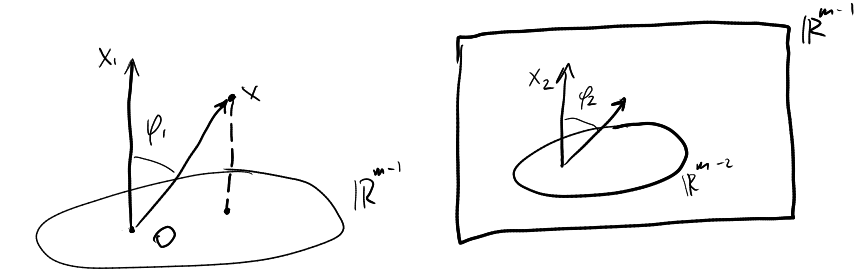
\includegraphics[scale=0.5]{6_1.png}
\end{center}
\[ x_1 = r\cos\varphi_1 \]
\[ x_2 = r \sin \varphi_1\cos\varphi_2 \]
\[ x_3 = 2 \sin \varphi_1 \sin\varphi_2 \cos\varphi_3 \]
\[ \vdots \]
\[ x_{m - 1} = r\sin\varphi_1 \dots \sin\varphi_{m - 2}\cos\varphi_{m - 1} \]
\[ x_m = r \sin\varphi_1 \dots \sin\varphi_{m - 2} \sin \varphi_{m - 1} \]
\[ J = r^{m - 1}\sin^{m - 2}\varphi_1\sin^{m - 3}\varphi_2 \dots \sin\varphi_{m - 2}\footnote{\text{В }\R^3\text{ ``географические`` координаты }J = r^2\cos\psi} \]
Сделаем в цикле эти координаты:
\begin{description}
\item[{шаг 1}] \(x_m = \rho_{m - 1}\sin\varphi_{m - 1}\) \\
\(x_{m - 1} = \rho_{m - 1}\cos\varphi_{m - 1}\) \\
\((x_1\ \dots\ x_n) \rightsquigarrow (x_1\ \dots\ x_{m - 2},\ \rho_{m - 1},\ \varphi_{m - 1})\)
\item[{шаг 2}] \(\rho_{m - 1} = \rho(m_2) \sin\varphi_{m - 2}\) \\
\(x_{m - 2} = \rho_{m - 2} \cos\varphi_{m - 2}\) \\
\((x_1\ \dots\ x_{m - 2},\ \rho_{m - 1},\ \varphi_{m -1}) \rightsquigarrow (x_1\ \dots\ x_{m - 3},\ \rho_{m - 2},\ \varphi_{m - 2},\ \varphi_{m - 1})\)
\item[{\(\vdots\)}] 

\item[{последний шаг}] \((x_1,\ \rho_2,\ \varphi_2\ \dots\ \varphi_{m - 1}) \rightsquigarrow (r,\ \varphi_1\ \dots\ \varphi_{m - 1})\) \\
\(\rho_2 = r\sin\varphi_1\) \\
\(x_1 = r \cos\varphi_1\)
\end{description}
\[ \lambda_m(\Omega) = \int\limits_\Omega 1 d\lambda_m \xlongequal[\text{1 шаг}]{} \int\limits_{\Omega_1} \rho_{m - 1} \xlongequal[\text{2 шаг}]{} \int\limits_{\Omega_2} \rho^2_{m - 2} \sin\varphi_{m - 2} \xlongequal[\text{3 шаг}]{} \int\limits_{\Omega_3} \rho^3_{m - 3} \sin^2\varphi_{m - 3}\sin\varphi_{m - 2} d\lambda = \]
\[ = \dots = \int\limits_{\Omega_{m - 1}}r^{m - 1}\sin^{n - 2}\varphi_{1} \dots \sin\varphi_{m - 2}\]
\end{examp}
\section{Произведение мер}
\label{sec:orgd2f5a59}
\begin{itemize}
\item \((X, \A, \mu)\)
\item \((Y, \B, \nu)\)
\end{itemize}
\begin{lemma}
\(\A, \B\) --- п/к \(\Rightarrow\) \(\A \times \B = \{A\times B \subset X \times Y | A \in \A,\ B\in\B\}\)
\end{lemma}
\begin{examp}
Ячейки: В \(\R^2 = \R^1 \times \R^1\ \A = \mathcal{P}^1,\ \B \in \mathcal{P}^1\) \\
\(A \times B\) --- ячейка из \(\mathcal{P}\)
\end{examp}
\begin{definition}
\(\mathcal{P} = \A \times \B\) --- множества из этой системы называются измеримыми прямоуг. \(m_o(A \times B) = \mu A\cdot \nu B\)
\end{definition}
\begin{theorem}
\-
\begin{enumerate}
\item \(m_0\) --- мера на \(\mathcal{P}\)
\item \(\nu,\mu\) --- \(\sigma\)-конечные \(\Rightarrow\) \(m_0\) --- тоже \(\sigma\)-конечная
\end{enumerate}
\end{theorem}
\begin{proof}
\-
\begin{enumerate}
\item ?\(m_0\) --- счетно аддитивна ?\(m_0 P = \sum m_o P_k\), если
\[ A \times B = P = \bigsqcup P_k\text{, где }P_k=A_k\times B_k \]
Наблюдение: \(\chi_{A \times B}(x, y) = \chi_A(x)\cdot\chi_B(y)\) \\
Тогда \(\chi_P = \sum \chi_{P_k}\), т.е.
\[ \forall x \in X, y \in Y\quad\chi_A(x)\chi_B(y) = \sum \chi_{A_k}(x)\chi_{B_k}(y) \]
проинтегрируем по \(y\) по мере \(\nu\):
\[ \chi_A(x) \nu B = \sum \chi_A(x)\cdot \nu B_k \]
Интегрируем по \(x\):
\[ \mu A \cdot \nu B - \sum \mu A_k \cdot \nu B_k  \]
\item Очев. \(\mu\) --- \(\sigma\)-конечная \(\Rightarrow\) \(X = \bigcup X_k\), \(\mu X_k\) --- конечная
\(nu\) --- \(\sigma\)-конечная \(\Rightarrow\) \(Y = \bigcup Y_n\), \(\nu Y_k\) --- конечная
\[ X \times Y = \bigcup X_k \timesy Y_n\quad m_0 \mu X_k \nu Y_n\text{ --- конечная} \]
\(\Rightarrow\) \(m_0\) --- \(\sigma\)-конечная мера
\end{enumerate}
\end{proof}
\begin{definition}
\-
\begin{itemize}
\item \((X, \A, \mu)\), \((Y, \B, \nu)\) --- пространства с мерой
\item \(\mu, \nu\) --- \(\sigma\)-конечные
\end{itemize}
Пусть \(m\) --- лебеговское продолжение меры \(m_0\) с п/к \(\A \times \B\) на \(\sigma\)-алгебра, которую будет обозначать \(\A \otimes \B\)
\end{definition}
\begin{definition}
\((X \times Y, \A \otimes \B, \nu \times \mu)\) --- произведение пространств с мерой \((X, \A, \mu)\) и \((Y, \B, \nu)\)
\end{definition}
\begin{remark}
\-
\begin{enumerate}
\item Это произведение ассоциативно
\item \(\sigma\)-конечность нужна для единственности произведения
\end{enumerate}
\end{remark}
\begin{theorem}
\(\lambda_m \times \lambda_n = \lambda_{n + m}\)
\end{theorem}
\begin{proof}
\color{red}Без доказательсва\color{black}
\end{proof}
\begin{definition}
\-
\begin{itemize}
\item \(X, Y\) --- множества
\item \(C \subset X \times Y\)
\end{itemize}
\[ C_x := \{y \in Y| (x, y) \in C\} \]
\[ C^y := \{x \in X| (x, y) \in C \} \]
\end{definition}
\begin{remark}
\[ \left(\bigcup\limits_\alpha C_\alpha\right)_x = \bigcup\left(C_\alpha\right)_x \]
\[ \left(\bigcap\limits_\alpha C_\alpha\right)_x = \bigcap\limits_\alpha\left(C_\alpha\right)_x \]
\[ \left(C \setminus C'\right)_x = C_x \setminus C'_x \]
\end{remark}
\begin{theorem}[Кавальери]
\-
\begin{itemize}
\item \((X, \A, \mu)\)
\item \((Y, \B, \nu)\)
\item \(\nu, \mu\) --- \(\sigma\)-конечные, полные
\item \(m := \mu \times \nu\)
\end{itemize}
Пусть \(C \in \A \otimes \B\) \\
\uline{Тогда}:
\begin{enumerate}
\item \(C_x \in \B\) при почти всех \(x\)
\item \(x \mapsto \nu(C_x)\) --- измеримая\footnote{функция задана при почти всех \(x\). Она равна почти везде некоторой измеримой функции, которая задана на всем \(X\). Это ``не мешает`` утверждению 3} функция на \(X\)
\item \(mC = \int\limits_X \nu(C_x)d\mu(x)\)
\end{enumerate}
Аналогичное верно для \(C^y\)
\end{theorem}
\begin{examp}
Половину шара сопоставляем с конусом.
\begin{center}
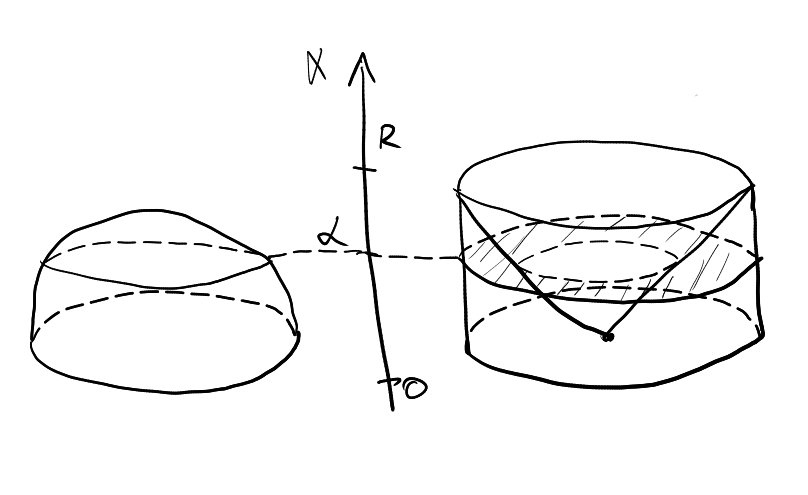
\includegraphics[scale=0.4]{6_2.png}
\end{center}
\begin{itemize}
\item \(C_x=\)круг
\item \(C_x=\)кольцо
\end{itemize}
\[ \lambda(C_x) = \pi(R^2 - x^2) \]
\[ \lambda(C_x) = \pi R^2 - \pi x^2 \]
\[ \nu(\frac{1}{2}\text{шара}) = \nu(\text{цилиндр}-\text{конус}) = \pi R^2 - \frac{1}{3} \pi R^2 = \frac{2}{3} \pi R^ \]
\end{examp}
\begin{proof}
\(\mathcal{D}\) --- система множеств, для которых выполнено 1. - 3. 
\begin{enumerate}
\item \(C = A\times B \Rightarrow C \in \mathcal{D}\)
\begin{enumerate}
\item \(C_x = \left[\begin{matrix} \emptyset & x \not\in A \\ B & x \in A\end{matrix}\right.\)
\item \(x \mapsto \nu(x)\) --- это функция \(\nu B \cdot \chi_A\)
\item \(\int \nu(C_x) d\mu = \int\limits_X \nu B \cdot \chi_A d\mu = \nu B \cdot \mu A = mC\)
\end{enumerate}
\item \(E_i \in D\), dis \(\Rightarrow\) \(\bigsqcup E_i \in D\) \\
\(E_i \in D \Rightarrow (E_i)_X\) --- измеримое почти везде \(\Rightarrow\) при почти всех \(x\) все \((E_i)_X\) -- измеримое \\
\begin{enumerate}
\item Тогда при этих \(x\ E_X = \bigsqcup(E_i)_X \in \B\)
\item \(\nu E_X = \sum \underbrace{\nu(E_i)_X}_\text{измеримая функция}\) \(\Rightarrow\) функция \(x \mapsto \nu E_X\) измеримая\(\footnotemark[\value{footnote}]\)
\item \[ \int\limits_X \nu E_X d\mu = \sum_i \int\limits_X \nu(E_i)_X = \sum_i mE_i = mE \]
\end{enumerate}
\item \(E_i \in \mathcal{D},\ E_1 \supset E_2 \supset \dots,\ E = \bigcap\limits_iE_i,\ \mu E_i < + \infty\) Тогда \(E \in \mathcal{D}\)
\[ \int\limits_X \nu(E_i)_X d\mu = mE_i < +\infty \Rightarrow \nu(E_i)_X\text{ --- конечная при почти всех }x \]
\begin{enumerate}
\item \(\forall x\) верно \((E_1)_X \supset (E_2)_X \supset \dots ,\ E_X = \bigcap (E_i)_X\). Тогда \(E_X\) --- измеримое при почти всех \(x\) и \(\lim\limits_{i \to + \infty} \nu(E_i)_X = \nu E_X\) при почти всех \(x\)
\item Таким образом \(x \mapsto \nu E_X\) --- измеримая\(\footnotemark[\value{footnote}]\)
\item \[ \int\limits_X \nu E_X d\mu = \lim \int \nu(E_i)_X d\mu = \lim mE_i = mE \]
Первое равенство по теореме Лебега о предельном переходе под знаком интеграла: \(|\nu (E_i)_X| \le \nu (E_1)_X\) --- из\(\footnotemark[\value{footnote}]\)
\end{enumerate}
\end{enumerate}
Итог: \(A_{ij} \in \mathcal{P} = \A \times \B\), то \(\color{red}??\color{black}\bigcup A_{ij} \in \mathcal{D}\)
\begin{enumerate}
\setcounter{enumi}{3}
\item \(mE = 0 \Rightarrow E \in \mathcal{D}\)
\[ mE = \inf\{\sum m_0 P_k | E \subset \bigcup P_k,\ P_k \in \mathcal{P}\} \]
--- теорема о лебеговском продолжении. \\
\(\exists\) множества \(H\) вида \(\bigcap\limits_e\bigsqcup\limits_X P_{ke}\) (т.е. \(H \in \mathcal{D}\)) \\
\(E \subset H, mH = mE = 0\)
\[ 0 = mH = \int\limits_X \nu H_x d\mu \Rightarrow \nu H_X \sim 0\text{ (\(=0\) при почти всех \(x\))} \]
\(E_X \subset H_x, \nu\) --- полная \(\Rightarrow\)
\begin{enumerate}
\item \(E_X\) --- измерима при почти всех \(x\)
\item \(\nu E_X = 0\) почти везде
\item \(\int \nu E_X d\mu = 0 = m E\)
\end{enumerate}
\item \(C\) --- \(m\)-измеримо, \(mC < + \infty\) тогда \(C \in \mathcal{D}\) \\
\(C = H \setminus e\), где \(H\) --- вида \(\color{red}???\color{black}\bigcup P_{ke},\ me = 0,\ mC = mH\)
\begin{enumerate}
\item \(C_x = H_x \setminus e_X\) --- измерима при почти всех \(x\), т.к. \(\nu\) --- полная
\item \(\nu e_X = 0\) при почти всех \(x\) \(\Rightarrow\) \(\nu C_x = \nu H_x - \nu e_X = \nu H_X\) \(\Rightarrow\) измерима
\item \(\int\limits_X \nu C_x d\mu = \int\limits_X \nu H_x d\mu = mH = mC\)
\end{enumerate}
\item \(C\) --- произвольное измеримое множество в \(X \times Y\) \(\Rightarrow\) \(C \in \mathcal{D}\) \\
\[ X = \bigsqcup X_k,\ \mu X_k < + \infty,\ Y = \bigsqcup Y_j,\ \nu Y_j < + \infty \]
\[ C = \bigsqcup (C \cap (X_k \times Y_j))\text{ --- используем 2.}\]
\end{enumerate}
\end{proof}
\begin{corollary}
\(C\) --- измеримое в \(X\times Y\). Пусть \(P_q(C) = \{x \in X| C_x \neq 0\}\) --- проекция \(C\) на \(X\). Если \(P_1(C)\) --- измеримое, то:
\[ mC = \int\limits_{P_1(C)} \nu(C_x) d\mu \]
\end{corollary}
\begin{proof}
при \(x \not\in P_1(C)\ \nu(C_x) = 0\)
\end{proof}
\begin{remark}
\-
\begin{enumerate}
\item \(С\) --- измеримое \(\not\Rightarrow\) \(P_1(C)\) --- измеримое
\item \(C\) --- измеримое \(\not\Rightarrow\) \(\forall x\ C_x\) --- измеримо
\item \(\forall x\forall y\ C_x,C^y\) --- измеримые \(\not\Rightarrow\) \(C\) --- измеримое (пример Серпинского)
\end{enumerate}
\end{remark}
\chapter{}
\label{sec:org35ebece}
\newcommand{\X}{\chi}
\newcommand{\A}{\mathfrak{A}}
\newcommand{\B}{\mathfrak{B}}
\newcommand{\M}{\mathfrak{M}}

\section{Принцип Кавальери}
\label{sec:org4a40e8d}
\begin{enumerate}
\item \(C_x\) --- имзмерима при почти всех \(x\)
\item \(x \mapsto \nu C_x\) --- измерима*
\item \(mC = \int\limits_X \mathcal{X}_x d\mu\)
\end{enumerate}
\begin{corollary}
\(f: [a, b] \to \R\) --- непрерывная \\
\uline{Тогда} \(\int\limits_a^b f(x)\,dx = \int\limits_{[a, b]} f\,d\lambda_1\)
\end{corollary}
\begin{proof}
\(f>0\ \text{ПГ}(f[a, b])\) --- измеримое множество в \(\R^2\). \(C_x = [0, f(x)]\ \lambda_1(C_x) = f(x)\)
\[ \int\limits_a^b f(x)\, dx = \lambda_2(\text{ПГ}) = \int\limits_{[a, b]} f d\lambda_1 \]
\end{proof}
\begin{remark}
\(\lambda_2\) можно продолжить на множество \(2^{\R^2}\) с сохранением свойства конечной аддитивности и это продолжение не единственно
\label{orgcbb7c36}
\end{remark}
\begin{remark}
\(\lambda_m, m>2\) --- аналогичным образом продолжить невозможно. Парадокс Хаусдорфа-Банаха-Тарского
\label{org624686f}
\end{remark}
\begin{remark}
Для \hyperref[orgcbb7c36]{замечания 1} и \hyperref[org624686f]{замечания 2} требуется инвариантность меры относительно движения \(\R^m\)
\end{remark}

\begin{definition}
\-
\begin{itemize}
\item \(C \subset X \times Y\)
\item \(f: X \times T \to \Y\)
\item \(\forall x \in X\ f_x\) --- это функция(сечение) \(f_x(y) = f(x, y)\), можно считать что она задана на \(C_x\)
\item \(f^y\) --- аналогичное сечение
\end{itemize}
\end{definition}
\begin{theorem}
\-
\begin{itemize}
\item \((X, \A, \mu)\)
\item \((Y, \B, \nu)\)
\item \(\mu, \nu\) --- \(\sigma\)-конечныемера, полные
\item \(m = \mu x \nu\)
\item \(f: X \times Y \to \overline{R}, f \ge 0\) --- измерима относительно \(A\otimes B\)
\end{itemize}
\uline{Тогда}
\begin{enumerate}
\item при  почти всех \(x\) \(f_x\) --- измеримая на \(Y\) \color{blue}\(f^y\) --- измерима на \(X\) почти везде\color{black}
\item \(x \mapsto \varphi(x)=\int\limits_Y f_x d\nu = \int\limits_Y f(x, y) = d\nu(y)\) --- измеримая* на \(X\) \\
\color{blue}\(y \mapsto \psi(y) = \int\limits_X f^y d\mu\) --- измеримая* на \(Y\)\color{black}
\item \(\int\limits_{X \times Y} d fm = \int\limits_X \varphi d\mu = \int\limits_X\left(\int\limits_Y f(x, y) d\nu(y)\right)d\mu(x)\) \\
\color{blue}\(= \int\limits_Y \psi d\nu = \int\limits_Y\left(\int\limits_X f(x, y) d\mu(x)\right)d\nu(y)\)
\end{enumerate}
\end{theorem}
\begin{proof}
\todo
\end{proof}
\begin{corllary}
\(C \subset X \times Y\) \(P_1(C)\) --- измеримо. \\
\uline{Тогда} \[ \int\limits_C f dm = \int\limits_{f_1(C)}\left(\int_{C_x} f(x, y) d\nu(y)\right)d\mu(x) \]
\end{corllary}
\begin{theorem}[Фубини]
\-
\begin{itemize}
\item \((X, \A, \mu)\)
\item \(Y, B, \nu\)
\item \(\nu, mu\) --- \(\sigma\)-конечные
\item \(m = \nu \times \mu\)
\item \(f\) --- суммируема на \(X \times Y\) относительно \(m\)
\end{itemize}
\uline{Тогда}
\begin{enumerate}
\item \(f_x\) --- суммируема на \(Y\) при почти всех \(x\)
\item \(x \mapsto \varphi(x) = \int_Y fx\,d\nu = \int_Y f(x, y)\,d\nu(y)\) --- суммируема на \(Y\)
\item \(\int\limits_{X \times Y} f\,dm = \int\limits_X \varphi\,d\mu = \int_X \left(\int_Y f(x, y) d\nu(y)\right) d\mu(x)\)
\end{enumerate}
\end{theorem}
\begin{proof}
\color{green}Без доказательства\color{black}
\end{proof}
\todo
\section{Поверхностные интегралы}
\label{sec:org5c53b4a}
\subsection{Поверхностные интегралы I рода}
\label{sec:org9081b64}
\begin{definition}
\(M \subset \R^3\) --- простое двумерное гладкое многообразие. \(\varphi: G \subset \R^2 \to \R^3\) --- параметризация. \(E \subset M\) --- измеримо по Лебегу, если \(\varphi^{-1}(E)\) измеримо в \(\R^2\) по Лебегу
\end{definition}
\begin{symb}
\(\A_M = \{E \subset M | E\text{ --- измеримо}\} = \{\varphi(A) | A \in \M^2,\ A \subset G\}\)
\end{symb}
\begin{definition}
Мера на \(\A_M\) \[S(E) := \iint\limits_{\varphi^{-1}(E)} | \varphi'_u \times \varphi'_v |\,dudv\]
Т.е. это взвешенный образ меры Лебега при отображении \(\varphi\)
\end{definition}
\begin{remark}
\(\A_M\) --- \(\sigma\)-алгебра, \(S\) --- мера
\end{remark}
\begin{remark}
\(E \subset M\) --- компактное \(\Rightarrow\ \varphi^{-1}(E)\) --- компактное \(\Rightarrow\) измеримое \(\Rightarrow\) замкнутые множества измеримы \(\Rightarrow\) (относительно) открытые множества измеримы
\end{remark}
\begin{remark}
\(\A_M\) не зависит от \(\varphi\) по теореме о двух параметризациях
\end{remark}
\begin{remark}
\(S\) не зависит от \(\varphi\)
\[ |\overline{\varphi'_s}\times\overline{\varphi'_v}| = |(\overline{\varphi'_s}\cdot u'_s + \overline{\varphi'_v}\cdot v'_s) \times (\overline{\varphi'_u}\cdot u'_t + \overline{\varphi'_v}\cdot v'_t)| = \]
\[ = | \overline{(\varphi'_u \times \varphi'_v)}\cdot(u'_s\cdot v'_t - v'_s\cdot u'_t)| = \todo \]
\end{remark}
\begin{remark}
\-
\begin{itemize}
\item \(f: \M \to \overline{R}\) --- измеримая
\end{itemize}
\(M(f<a)\) --- измеримая \(\Leftrightarrow\) \(N(f\circ\varphi<a)\) --- измерима относително \(\M^2\) \\
\(f\) --- измерима относительно \(\A_M\) \(\Leftrightarrow\) \(f \circ \varphi\) --- измерима относительно \(\M^2\)
\end{remark}
\begin{definition}[поверхностный интеграл I рода]
\-
\begin{itemize}
\item \(M\) --- простое гладкое двумерное иногообразие в \(\R^3\)
\item \(\varphi\) --- параметризация
\item \(f: M \to \overline{R}\) --- суммируема по мере \(S\)
\end{itemize}
То \[ \iint\limits_M f\,ds = \iint\limits_M f(x, y, z)\,ds \]
называется \textbf{интегралом I рода от \(f\) по многообразию \(M\)}
\end{definition}
\begin{remark}
По теореме об интегрировании по взвешенному образу меры
\[ \iint\limits_M f\,ds = \iint\limits_G f(\varphi(u, v)) |\varphi'_v \times \varphi'_v|\,dudv \]
\[ \varphi'_u \times \varphi'_v = \begin{pmatrix}
i & x'_u & x'_v \\
j & y'_u & y'_v \\
k & z'_u & z'_v
\end{pmatrix}\]
\[ |\varphi'_u \times \varphi'_v| = |\varphi'_u| \cdot |\varphi'_v|\sun\alpha = \sqrt{|\varphi'_u|^2 \cdot |varphi'_v|^2 \cdot (1 - \cos^2\alpha)} = \sqrt{EG - F^2} \]
\[ E = |\varphi'_u| = x'_u^2 + y'_u^2 + z'_u^2 \]
\[ F = \langle \varphi'_u, \varphi'_v \rangle = x'_ux'_v + y'_uy'_v + z'_u z'_v \quad F = |\varphi'_v|^2 \]
\end{remark}
\chapter{5 апреля}
\label{sec:orgc7c5985}
\newcommand{\A}{\mathfrak{A}}
\newcommand{\esssup}{\mathop{\rm ess\,sup}\limits}


\begin{itemize}
\item \(M\)
\item \(\Phi: O \subset \R^2 \to \R^3\)
\item \(f\)
\item \(f \citc \Phi\)
\end{itemize}
\[ \int_{M/E} d fs = \int_{O/\Phi^{-1}(E)} f \circ \Phi \cdot |\Phi'u\times\Phi'v|\,du\,dv \]
\begin{definition}
\(M \subset \R^3\) --- \textbf{кусочно гладкое двумерное многообразие}, если
\(M\) --- конечное объединение
\begin{itemize}
\item простых гладких двумерных многообразий \(M_i\)
\item гладких кривых
\item точек
\end{itemize}
\end{definition}
\begin{remark}
Просто так сферу параметризовать не можем, но можем разбить ее на две полусферы и окружность и считать отдельно для каждой из них.
\end{remark}
\begin{definition}
\(E \subset M\) --- измеримое, если измеримы все \(E \cap M_i\). \\
\[S(E) := \sum_i S(E\cap M_i) \]
\[ \int_E f ds := \sum_i \int_{E \cap M_i} f ds \]
\end{definition}
\section{Поверхностный интеграл II рода}
\label{sec:org47fc054}
\begin{itemize}
\item \(M\) --- простое гладкое двумерное многообразие в \(R^3\) --- поверхность
\end{itemize}
\begin{definition}
\textbf{Сторона поверхности} --- непрерывное семейство единичных нормалей к этой поверхности \\
\(M \subset \R^3 \quad W: M \to \R^3\) \\
\(\forall x\ W(x)\) --- нормаль к \(M\), \(|w(x)| = 1\), \(w(x) \perp \Phi'u,\Phi'_v\)
\end{definition}
\begin{remark}
Локльно каждая повехность --- двустороннее. В общем случае --- 1 или 2 стороны
\end{remark}
\begin{remark}
График функции \(z(x, y)\)
\[ \Phi: (x, y) \mapsto \begin{pmatrix} x \\ y \\ z(x, y) \end{pmatrix} \]
\[ \Phi'_x = \begin{pmatrix} 1 \\ 0 \\ z'_x \end{pmatrix}\quad\Phi'_y = \begin{pmatrix} 0 \\ 1 \\ z'_y \end{pmatrix} \]
--- касательные векторы
\[n := \Phi'_x \times \Phi'_y = \begin{pmatrix} -z'_x \\ -z'_y \\ 1 \end{pmatrix}\] --- нормаль
\[ n_0 = \pm \left(-\frac{z'_x}{\sqrt{1 + z'_x^2 + z'_y^2}}, -\frac{z'_y}{\sqrt{\dots}}, \frac{1}{\sqrt{\dots}}\right) \]
\end{remark}
\begin{remark}
Другой способ задания стороны поверхности
\begin{enumerate}
\item \(u, v\) --- касательные векторы \\
\(u \not\parallel v\), \((u, v)\) --- касательный реп\(\acute{\text{е}}\)р \\
Если задано непрерывное поле реперов, то они задают сторону \(n = u \times v\)(отнормировать)
\item Задана петля + указано непрерывное движение
\end{enumerate}
\end{remark}
\begin{definition}
\(M\) --- поверхность в \(\R^3\), \(n_0\) --- сторона, \(\gamma\) --- контур(петля) в \(M\) --- ориентированный. \\
Говорят, что сторона поверхности \(n_0\) согласована с ориентацией \(\gamma\): \((\gamma' \times N_\text{внутр.}) \parallel n_0\). Т.е. если ориентация \(\gamma\) задает сторону \(n_0\)
\end{definition}
\begin{definition}
\-
\begin{itemize}
\item \(M\) --- простое двумерное гладкое многообразие
\item \(n_0\) --- сторона \(M\)
\item \(F: M \to \R^3\) --- векторное поле(непрерывное)
\end{itemize}
\[ \int_M \langle F, n_0 \rangle \, ds \] --- \textbf{интеграл II рода} векторного поля \(F\) по поверхности \(M\)
\end{definition}
\begin{remark}
Смена стороны = смена знака
\end{remark}
\begin{remark}
Не зависит от параметра
\end{remark}
\begin{remark}
\(F = (P, Q, R)\) обозначается
\[ \iint_M P \, dy\,dz + Q\,dz\,dx + R\,dx\,dy \]
\end{remark}
\begin{remark}
\(\Phi, n = \Phi'_u \times \Phi'_v \leadsto n_0\)
\[ \int_M \langle F, n_0 \rangle = \int_O \left\langle F, \frac{\Phi'_u \times \Phi'_v}{|\Phi'_u\times\Phi'_v} \right\rangle |\Phi'_u\times\Phi'_v|\,du\,dv =  \]
\[ \int_O \underbrace{\langle F, \Phi'_u\times\Phi'_v \rangle}_\text{смешенное произведение} \,du\,dv \addtag\label{int_1_8} \]
\[ \Phi(u, v) = (x(u, v), y(u, v), z(u, v)) \]
\[ \langle F, \Phi'_u\times\Phi'_v \rangle = \det\begin{pmatrix}P & x'_u & x'_v \\ Q & y'_u & y'_v \\ R & z'_u & z'_v\end{pmatrix} \]
\[ \ref{int_1_8} = \int_O P\cdot\begin{vmatrix} y'_u & z'_v \\ z'_u & z'_v \end{vmatrix} + Q\cdot\begin{vmatrix}z'_u & z'_v \\ x'_u & x'_v\end{vmatrix} + R\cdot\begin{vmatrix}x'_u & x'_v \\ y'_u & y'_v\end{vmatrix}\,du\,dv \]
\end{remark}
\begin{examp}
График \(z(x, y)\) над областью \(G\) по верхней стороне
\[ \iint_{\Gamma_z} R\,dx\,dy = \iint_{\Gamma_z} 0\,dy\,dz + 0\,dz\,dy + R(x, y, z)\,dx\,dy \addtag\label{int_2_8} \]
\[ n_0 = \left(-\frac{z'_x}{\sqrt{1 + z'_x^2 + z'_y^2}}, -\frac{z'_y}{\sqrt{\dots}}, \frac{1}{\sqrt{\dots}}\right) \]
\[ \ref{int_2_8} = \iint_{\Gamma_z} R(x, y, z)\cdot \frac{1}{\sqrt{1 + z'_x^2 + z'_y^2}}\,ds = \iint_G R(x, y, z(x, y)) \,dx\,dy = \iint_G R\,dx\,dy \]
т.е. этот интеграл II рода равен интегралу по проекции
\end{examp}
\begin{corollary}
\-
\begin{itemize}
\item \(V \subset \R^3\)
\item \(M = \partial V\) --- гладкая двумерная поверхность
\item \(n_0\) --- внешняя нормаль
\end{itemize}
\[ \lambda_3 V = \iint_{\partial V} z\,dx\,dy = \frac{1}{3}\iint_{\partial V} x\,dy\,dz + y\,dz\,dx + z\,dx\,dy \]
\end{corollary}
\begin{corollary}
\(\Omega\) --- гладкая кривая в \(\R^2\), \(M\) (--- цилиндр над \(\Omega\)) \(=\Omega \times [z_0, z_1]\) \\
\uline{Тогда} (сторона \(M\) любая) \(\int_M R\,dx\,dy = 0\)
\end{corollary}
\section{Ряды Фурье}
\label{sec:orgb316bec}
\subsection{Пространства \(L^p\)}
\label{sec:org2072e13}
\begin{property}
\-
\begin{itemize}
\item \((X, \A, \mu)\)
\item \(f: X \to \C\) \\
\(x = f(x) = u(x) + iv(x)\) \\
\(u = \Re f,\ v = \Im f\) \\
\item \(f\) --- измеримая, если \(u\) и \(v\) --- измеримые
\item \(f\) --- суммируемая, \(u\) и \(v\) --- суммирумые
\item \(f\) --- суммируемая: \(\int_E f = \int_E u + \int_E v\)
\end{itemize}
\end{property}
\begin{property}[Неравенство Гёльдера]
\-
\begin{itemize}
\item \(p,q > 1\) \(\frac{1}{p} + \frac{1}{q} = 1\)
\item \((X, \A, \mu)\)
\item \(E\) --- измеримое
\item \(f, g: E \to \C\) --- измеримые
\end{itemize}
\uline{Тогда} \[ \int_E |fg| d\mu \le \left(\int_E |f|^p\right)^{\frac{1}{p}} \left(\int_E |g|^q\right)^{\frac{1}{q}} \]
\label{orga46c7c8}
\end{property}
\begin{property}[Неравенство Минковского]
Те-же условия что и в \hyperref[orga46c7c8]{Неравенстве Гельдера}
\[ \left(\int_E |f + g|^p\right)^{\frac{1}{p}} \le \left(\int_E |f|^p\right)^{\frac{1}{p}} + \left(\int_E |g|^p\right)^{\frac{1}{p}} \]
\end{property}
\begin{remark}
При \(p = 1\) неравенство тоже верно
\end{remark}
\begin{property}
\begin{definition}
\(L^p\), \(1 \le p \le +\infty\)
\begin{itemize}
\item \((X, \A, \mu)\)
\item \(E \subset X\) --- измеримое
\end{itemize}
\[ \mathcal{L}^p(E, \mu) := \left\{f: \text{ почти везде }E \to \R(\C) \Big| f\text{ --- измеримая}, \int_E |f|^p\,d\mu < +\infty\right\} \]
--- это линейное пространство (по неравенству Минковского) \\
\(f, g \in \mathcal{L}^p(E, \mu): f \sim g\quad f = h\text{ почти везде}\). \(\mathcal{L}^p/_N = L^p(E, \mu)\) --- линейной пространство. Задаем норму \(\Vert f \Vert_{L^p(E, \mu)} = \left(\int_E |f|^p\right)^{\frac{1}{p}}\)
\end{definition}
\end{property}

\begin{property}
\-
\begin{itemize}
\item \(L^\infty(E,\mu)\)
\item \((X, \A, \mu)\)
\item \(E\) --- измеримое
\item \(f\) --- почти везде \(E \to \overline{\R}\) --- измеримая
\end{itemize}
\[ \esssup_{x \in E} f = \inf \{A \in \overline{R}\Big| f \le A\text{ почти везде}\} \]
\end{property}
\beginproperties
\begin{property}
\(\esssup f \le \sup f\)
\end{property}
\begin{property}
\(f \le \esssup f\) почти везде
\end{property}
\begin{proof}
\(B = \esssup f\) \\
Тогда 
\end{proof}

\begin{property}
\(f\) --- сумм, \(\esssup_E |g| < +\infty\) \\
\uline{Тогда} \[ \left| \int_E fg \right| \le \esssup |g| \cdot \int_E |f| \]
\end{property}
\begin{proof}
\[ \left| \int_E fg \right| \le \int_E |fg| \le \int_E \esssup |g|\cdot|f| \]
\end{proof}
\begin{remark}
\(L^\infty(E, \mu) = \{f: \text{п.в. } E \to \overline{\R}(\overline{\C}),\text{ изм.}, \esssup |f| < +\infty \}/_\sim\). Эквивалентные функции отождествленны --- это нормированное пространство
\[ \Vert f \Vert_{L^\infty(E, \mu)} := \esssup_E |f| = \Vert f \Vert_\infty \]
\end{remark}
\begin{remark}
В новых обозначениях. Неравенство Гельдера:
\[ \Vert fg \Vert_1 \le \Vert f \Vert_p \cdot \Vert g \Vert_q \]
Здесь можно брать \(p = 1,\ q = +\infty\)
\end{remark}
\begin{remark}
\(f \in L^p\) \(\Rightarrow\) \(f\) --- почти везде конечны. \(1 \le p \le +\infty\) \(\Rightarrow\) можно считать \(f\) --- задана всюду на \(E\), и всюду конечна
\end{remark}
\chapter{12 апреля}
\label{sec:orgd25b948}
\newcommand{\A}{\mathfrak{A}}
\newcommand{\esssup}{\mathop{\rm ess\,sup}\limits}


\begin{itemize}
\item \(M\)
\item \(\Phi: O \subset \R^2 \to \R^3\)
\item \(f\)
\item \(f \citc \Phi\)
\end{itemize}
\[ \int_{M/E} d fs = \int_{O/\Phi^{-1}(E)} f \circ \Phi \cdot |\Phi'u\times\Phi'v|\,du\,dv \]
\begin{definition}
\(M \subset \R^3\) --- \textbf{кусочно гладкое двумерное многообразие}, если
\(M\) --- конечное объединение
\begin{itemize}
\item простых гладких двумерных многообразий \(M_i\)
\item гладких кривых
\item точек
\end{itemize}
\end{definition}
\begin{remark}
Просто так сферу параметризовать не можем, но можем разбить ее на две полусферы и окружность и считать отдельно для каждой из них.
\end{remark}
\begin{definition}
\(E \subset M\) --- измеримое, если измеримы все \(E \cap M_i\). \\
\[S(E) := \sum_i S(E\cap M_i) \]
\[ \int_E f ds := \sum_i \int_{E \cap M_i} f ds \]
\end{definition}
\section{Поверхностный интеграл II рода}
\label{sec:org15fdded}
\begin{itemize}
\item \(M\) --- простое гладкое двумерное многообразие в \(R^3\) --- поверхность
\end{itemize}
\begin{definition}
\textbf{Сторона поверхности} --- непрерывное семейство единичных нормалей к этой поверхности \\
\(M \subset \R^3 \quad W: M \to \R^3\) \\
\(\forall x\ W(x)\) --- нормаль к \(M\), \(|w(x)| = 1\), \(w(x) \perp \Phi'u,\Phi'_v\)
\end{definition}
\begin{remark}
Локльно каждая повехность --- двустороннее. В общем случае --- 1 или 2 стороны
\end{remark}
\begin{remark}
График функции \(z(x, y)\)
\[ \Phi: (x, y) \mapsto \begin{pmatrix} x \\ y \\ z(x, y) \end{pmatrix} \]
\[ \Phi'_x = \begin{pmatrix} 1 \\ 0 \\ z'_x \end{pmatrix}\quad\Phi'_y = \begin{pmatrix} 0 \\ 1 \\ z'_y \end{pmatrix} \]
--- касательные векторы
\[n := \Phi'_x \times \Phi'_y = \begin{pmatrix} -z'_x \\ -z'_y \\ 1 \end{pmatrix}\] --- нормаль
\[ n_0 = \pm \left(-\frac{z'_x}{\sqrt{1 + z'_x^2 + z'_y^2}}, -\frac{z'_y}{\sqrt{\dots}}, \frac{1}{\sqrt{\dots}}\right) \]
\end{remark}
\begin{remark}
Другой способ задания стороны поверхности
\begin{enumerate}
\item \(u, v\) --- касательные векторы \\
\(u \not\parallel v\), \((u, v)\) --- касательный реп\(\acute{\text{е}}\)р \\
Если задано непрерывное поле реперов, то они задают сторону \(n = u \times v\)(отнормировать)
\item Задана петля + указано непрерывное движение
\end{enumerate}
\end{remark}
\begin{definition}
\(M\) --- поверхность в \(\R^3\), \(n_0\) --- сторона, \(\gamma\) --- контур(петля) в \(M\) --- ориентированный. \\
Говорят, что сторона поверхности \(n_0\) согласована с ориентацией \(\gamma\): \((\gamma' \times N_\text{внутр.}) \parallel n_0\). Т.е. если ориентация \(\gamma\) задает сторону \(n_0\)
\end{definition}
\begin{definition}
\-
\begin{itemize}
\item \(M\) --- простое двумерное гладкое многообразие
\item \(n_0\) --- сторона \(M\)
\item \(F: M \to \R^3\) --- векторное поле(непрерывное)
\end{itemize}
\[ \int_M \langle F, n_0 \rangle \, ds \] --- \textbf{интеграл II рода} векторного поля \(F\) по поверхности \(M\)
\end{definition}
\begin{remark}
Смена стороны = смена знака
\end{remark}
\begin{remark}
Не зависит от параметра
\end{remark}
\begin{remark}
\(F = (P, Q, R)\) обозначается
\[ \iint_M P \, dy\,dz + Q\,dz\,dx + R\,dx\,dy \]
\end{remark}
\begin{remark}
\(\Phi, n = \Phi'_u \times \Phi'_v \leadsto n_0\)
\[ \int_M \langle F, n_0 \rangle = \int_O \left\langle F, \frac{\Phi'_u \times \Phi'_v}{|\Phi'_u\times\Phi'_v} \right\rangle |\Phi'_u\times\Phi'_v|\,du\,dv =  \]
\[ \int_O \underbrace{\langle F, \Phi'_u\times\Phi'_v \rangle}_\text{смешенное произведение} \,du\,dv \addtag\label{int_1_8} \]
\[ \Phi(u, v) = (x(u, v), y(u, v), z(u, v)) \]
\[ \langle F, \Phi'_u\times\Phi'_v \rangle = \det\begin{pmatrix}P & x'_u & x'_v \\ Q & y'_u & y'_v \\ R & z'_u & z'_v\end{pmatrix} \]
\[ \ref{int_1_8} = \int_O P\cdot\begin{vmatrix} y'_u & z'_v \\ z'_u & z'_v \end{vmatrix} + Q\cdot\begin{vmatrix}z'_u & z'_v \\ x'_u & x'_v\end{vmatrix} + R\cdot\begin{vmatrix}x'_u & x'_v \\ y'_u & y'_v\end{vmatrix}\,du\,dv \]
\end{remark}
\begin{examp}
График \(z(x, y)\) над областью \(G\) по верхней стороне
\[ \iint_{\Gamma_z} R\,dx\,dy = \iint_{\Gamma_z} 0\,dy\,dz + 0\,dz\,dy + R(x, y, z)\,dx\,dy \addtag\label{int_2_8} \]
\[ n_0 = \left(-\frac{z'_x}{\sqrt{1 + z'_x^2 + z'_y^2}}, -\frac{z'_y}{\sqrt{\dots}}, \frac{1}{\sqrt{\dots}}\right) \]
\[ \ref{int_2_8} = \iint_{\Gamma_z} R(x, y, z)\cdot \frac{1}{\sqrt{1 + z'_x^2 + z'_y^2}}\,ds = \iint_G R(x, y, z(x, y)) \,dx\,dy = \iint_G R\,dx\,dy \]
т.е. этот интеграл II рода равен интегралу по проекции
\end{examp}
\begin{corollary}
\-
\begin{itemize}
\item \(V \subset \R^3\)
\item \(M = \partial V\) --- гладкая двумерная поверхность
\item \(n_0\) --- внешняя нормаль
\end{itemize}
\[ \lambda_3 V = \iint_{\partial V} z\,dx\,dy = \frac{1}{3}\iint_{\partial V} x\,dy\,dz + y\,dz\,dx + z\,dx\,dy \]
\end{corollary}
\begin{corollary}
\(\Omega\) --- гладкая кривая в \(\R^2\), \(M\) (--- цилиндр над \(\Omega\)) \(=\Omega \times [z_0, z_1]\) \\
\uline{Тогда} (сторона \(M\) любая) \(\int_M R\,dx\,dy = 0\)
\end{corollary}
\section{Ряды Фурье}
\label{sec:orga928b29}
\subsection{Пространства \(L^p\)}
\label{sec:org5d1d563}
\begin{property}
\-
\begin{itemize}
\item \((X, \A, \mu)\)
\item \(f: X \to \C\) \\
\(x = f(x) = u(x) + iv(x)\) \\
\(u = \Re f,\ v = \Im f\) \\
\item \(f\) --- измеримая, если \(u\) и \(v\) --- измеримые
\item \(f\) --- суммируемая, \(u\) и \(v\) --- суммирумые
\item \(f\) --- суммируемая: \(\int_E f = \int_E u + \int_E v\)
\end{itemize}
\end{property}
\begin{property}[Неравенство Гёльдера]
\-
\begin{itemize}
\item \(p,q > 1\) \(\frac{1}{p} + \frac{1}{q} = 1\)
\item \((X, \A, \mu)\)
\item \(E\) --- измеримое
\item \(f, g: E \to \C\) --- измеримые
\end{itemize}
\uline{Тогда} \[ \int_E |fg| d\mu \le \left(\int_E |f|^p\right)^{\frac{1}{p}} \left(\int_E |g|^q\right)^{\frac{1}{q}} \]
\label{org79c2b59}
\end{property}
\begin{property}[Неравенство Минковского]
Те-же условия что и в \hyperref[orga46c7c8]{Неравенстве Гельдера}
\[ \left(\int_E |f + g|^p\right)^{\frac{1}{p}} \le \left(\int_E |f|^p\right)^{\frac{1}{p}} + \left(\int_E |g|^p\right)^{\frac{1}{p}} \]
\end{property}
\begin{remark}
При \(p = 1\) неравенство тоже верно
\end{remark}
\begin{property}
\begin{definition}
\(L^p\), \(1 \le p \le +\infty\)
\begin{itemize}
\item \((X, \A, \mu)\)
\item \(E \subset X\) --- измеримое
\end{itemize}
\[ \mathcal{L}^p(E, \mu) := \left\{f: \text{ почти везде }E \to \R(\C) \Big| f\text{ --- измеримая}, \int_E |f|^p\,d\mu < +\infty\right\} \]
--- это линейное пространство (по неравенству Минковского) \\
\(f, g \in \mathcal{L}^p(E, \mu): f \sim g\quad f = h\text{ почти везде}\). \(\mathcal{L}^p/_N = L^p(E, \mu)\) --- линейной пространство. Задаем норму \(\Vert f \Vert_{L^p(E, \mu)} = \left(\int_E |f|^p\right)^{\frac{1}{p}}\)
\end{definition}
\end{property}

\begin{property}
\-
\begin{itemize}
\item \(L^\infty(E,\mu)\)
\item \((X, \A, \mu)\)
\item \(E\) --- измеримое
\item \(f\) --- почти везде \(E \to \overline{\R}\) --- измеримая
\end{itemize}
\[ \esssup_{x \in E} f = \inf \{A \in \overline{R}\Big| f \le A\text{ почти везде}\} \]
\end{property}
\beginproperties
\begin{property}
\(\esssup f \le \sup f\)
\end{property}
\begin{property}
\(f \le \esssup f\) почти везде
\end{property}
\begin{proof}
\(B = \esssup f\) \\
Тогда 
\end{proof}

\begin{property}
\(f\) --- сумм, \(\esssup_E |g| < +\infty\) \\
\uline{Тогда} \[ \left| \int_E fg \right| \le \esssup |g| \cdot \int_E |f| \]
\end{property}
\begin{proof}
\[ \left| \int_E fg \right| \le \int_E |fg| \le \int_E \esssup |g|\cdot|f| \]
\end{proof}
\begin{remark}
\(L^\infty(E, \mu) = \{f: \text{п.в. } E \to \overline{\R}(\overline{\C}),\text{ изм.}, \esssup |f| < +\infty \}/_\sim\). Эквивалентные функции отождествленны --- это нормированное пространство
\[ \Vert f \Vert_{L^\infty(E, \mu)} := \esssup_E |f| = \Vert f \Vert_\infty \]
\end{remark}
\begin{remark}
В новых обозначениях. Неравенство Гельдера:
\[ \Vert fg \Vert_1 \le \Vert f \Vert_p \cdot \Vert g \Vert_q \]
Здесь можно брать \(p = 1,\ q = +\infty\)
\end{remark}
\begin{remark}
\(f \in L^p\) \(\Rightarrow\) \(f\) --- почти везде конечны. \(1 \le p \le +\infty\) \(\Rightarrow\) можно считать \(f\) --- задана всюду на \(E\), и всюду конечна
\end{remark}
\end{document}
